\SGAchapter{XIV}{正则元素（续）：在代数群中的应用}{Éléments réguliers : suite, application aux groupes algébriques}
\SourcePage{219}
\begin{center}A.~Grothendieck\\附录由 J.-P.~Serre 撰写\end{center}
\footnote{原文版本记号：2008 年 12 月 1 日 xy 版。}
\SGAsection{1}{光滑代数群的 Cartan 子群与极大环面的构造}
\begin{SGAresult}{\Term{theorem}{定理}}{1.1}
设 $G$ 是域 $k$ 上的\Term{smooth}{光滑}\Term{algebraic-group}{代数群}。则 $G$ 有一个\Term{maximal-torus}{极大环面} $T$，因而有一个\Term{cartan-subgroup}{Cartan 子群} $C=\operatorname{Centr}_G(T)$。
\end{SGAresult}
根据第 XII 讲 3.2，在 $G$ 中寻找\Term{maximal-torus}{极大环面} $T$，与寻找\Term{cartan-subgroup}{Cartan 子群} $C$ 是一回事。此外，$G$ 的\Term{maximal-torus}{极大环面}就是 $G^0$ 的\Term{maximal-torus}{极大环面}，所以可以假定 $G$ \Term{connected}{连通}。我们分两种情形。

$1^\circ$）域 $k$ \Term{finite}{有限}。设 $\mathcal T$ 是 $G$ 的\Term{maximal-torus}{极大环面}\Term{scheme}{概形}（第 XII 讲 1.10），它在 $k$ 上\Term{smooth}{光滑}。注意，$G$ 通过\Term{inner-automorphism}{内自同构}\Term{action}{作用}于 $\mathcal T$；根据\Term{conjugacy}{共轭}\Term{theorem}{定理}（第 XII 讲 6.6 a)），$\mathcal T_{\bar k}$ 的任意两个 $\bar k$ \Term{rational-point}{有理点}在 $G_{\bar k}(\bar k)$ 的\Term{action}{作用}下互相对应。由于 $\mathcal T$ 在 $k$ 上\Term{smooth}{光滑}，从而 $\mathcal T_{\bar k}$ 在 $\bar k$ 上\Term{smooth}{光滑}，可知 $\mathcal T_{\bar k}$ \Term{isomorphism}{同构}于 $G_{\bar k}/N$，其中 $N$ 是 $\mathcal T_{\bar k}(\bar k)$ 中一个元素的\Term{stabilizer}{稳定子}，即 $G_{\bar k}$ 的某个\Term{maximal-torus}{极大环面} $T$ 的\Term{normalizer}{正规化子}。因此，$\mathcal T$ 是 $G$ \Term{action}{作用}下的一个“\Term{homogeneous-space}{齐性空间}”。Lang 的一个著名\Term{theorem}{定理}（\emph{Amer. J. Math.}\ \textbf{78}, 1956, pp.~555--563）告诉我们，\Term{finite-field}{有限域} $k$ 上\Term{smooth}{光滑}\Term{connected}{连通}\Term{algebraic-group}{代数群}的任意\Term{homogeneous-space}{齐性空间}都有\Term{rational-point}{有理点}。特别地，$\mathcal T$ 有一个\Term{rational-point}{有理点}，即 $G$ 有一个\Term{maximal-torus}{极大环面} $T$。证毕。

$2^\circ$）域 $k$ 无限。我们将使用下面的\Term{lemma}{引理}。
\begin{SGAresult}{\Term{lemma}{引理}}{1.2}
设 $G$ 是域 $k$ 上的\Term{smooth}{光滑}\Term{algebraic-group}{代数群}。则 $G$ 有一个\Term{type-c-subgroup}{(C) 型子群}（第 XIII 讲 6.2）。
\end{SGAresult}
根据第 XIII 讲 6.3，这\Term{equivalence}{等价}于说 $\mathfrak g$ 含有一个\Term{cartan-subalgebra}{Cartan 子代数} $\mathfrak d$。当 $k$ 无限时这是显然的，因为此时 $\mathfrak g$ 含有一个\Term{regular-element}{正则元素} $a$，取 $\mathfrak d=\operatorname{Nil}(a,\mathfrak g)$ 即可。$k$ \Term{finite}{有限}的情形可完全按照上面 $1^\circ$）中的证明处理，但须先构造 $\mathfrak g$ 的\Term{cartan-subalgebra}{Cartan 子代数}\Term{scheme}{概形} $\mathcal D$，并知道它在 $k$ 上\Term{smooth}{光滑}；这些将在下面证明（2.16）。
\SourcePage{220}
要在我们所处的 $2^\circ$）情形证明 1.1，无论如何只需知道无限域 $k$ 的情形下 1.2 成立。也顺便记下：
\begin{SGAresult}{\Term{lemma}{引理}}{1.3}
设 $G$ 是一个\Term{smooth}{光滑}\Term{connected}{连通}\Term{affine}{仿射}\Term{algebraic-group}{代数群}，其\Term{reductive-center}{约化中心}（第 XII 讲 4.1、4.4）是\Term{unit-group}{单位群}。则 $G$ \Term{nilpotent}{幂零}当且仅当它的\Term{lie-algebra}{Lie 代数} $\mathfrak g$ \Term{nilpotent}{幂零}。
\end{SGAresult}
这已包含在第 XII 讲 4.9 中。

现在可以给出构造 $G$ 的\Term{cartan-subgroup}{Cartan 子群}的方法（若承认\Term{finite-field}{有限域}情形的 1.2，此方法也适用于 $k$ \Term{finite}{有限}的情形）。先设 $G$ \Term{affine}{仿射}。对 $n=\dim G$ 归纳，$n=0$ 时断言显然。设 $n>0$，且已对所有 $n'<n$ 证明了断言。设 $Z$ 是 $G$ 的\Term{reductive-center}{约化中心}，令
\[u:G\longrightarrow G'=G/Z\]
为\Term{canonical-homomorphism}{典范同态}。根据第 XII 讲 4.7 c)，由 $C'\mapsto C=u^{-1}(C)$，$G'$ 的\Term{cartan-subgroup}{Cartan 子群}与 $G$ 的\Term{cartan-subgroup}{Cartan 子群}一一对应。因此，以 $G'$ 代替 $G$ 后，可以假定 $G$ 的\Term{reductive-center}{约化中心} $Z$ 只含单位元素（因为根据第 XII 讲 4.7 b)，$G'$ 的\Term{reductive-center}{约化中心}就是如此）。根据 1.3，$G$ 有一个\Term{type-c-subgroup}{(C) 型子群} $D$。我们知道，在 $k$ 的\Term{algebraic-closure}{代数闭包} $\bar k$ 上，$D_{\bar k}$ 含有 $G_{\bar k}$ 的一个\Term{cartan-subgroup}{Cartan 子群}（第 XIII 讲 6.6 b)），所以 $D$ 的任意\Term{cartan-subgroup}{Cartan 子群}都是 $G$ 的\Term{cartan-subgroup}{Cartan 子群}（第 XIII 讲 2.8 a)）。故问题归结为寻找 $D$ 的\Term{cartan-subgroup}{Cartan 子群}。若 $\dim D=\dim G$，即 $D=G$，则 $G$ 的\Term{lie-algebra}{Lie 代数}是其自身的\Term{cartan-subalgebra}{Cartan 子代数}，因而\Term{nilpotent}{幂零}；由 1.3，$G$ \Term{nilpotent}{幂零}，从而它是其自身的\Term{cartan-subgroup}{Cartan 子群}。若 $\dim D<\dim G$，则由归纳假设，$D$ 有一个\Term{cartan-subgroup}{Cartan 子群}，它也就是 $G$ 的\Term{cartan-subgroup}{Cartan 子群}。这就完成了 $G$ \Term{affine}{仿射}时的证明。一般情形下，设 $Z$ 是 $G$ 的\Term{center}{中心}，则 $G/Z=G'$ \Term{affine}{仿射}（第 XII 讲 6.1），且 $G'$ 的每个\Term{cartan-subgroup}{Cartan 子群} $C'$ 在 $G$ 中的\Term{inverse-image}{逆像} $C$ 都是 $G$ 的\Term{cartan-subgroup}{Cartan 子群}（第 XII 讲 6.6 e)）。这样就归结为在\Term{smooth}{光滑}\Term{affine}{仿射}\Term{algebraic-group}{代数群} $G'$ 中寻找\Term{cartan-subgroup}{Cartan 子群}，这个情形已经处理过。
\begin{SGAresult}{推论}{1.4}
设 $G$ 是 Artin \Term{scheme}{概形} $S$ 上\Term{finite-type}{有限型}的\Term{smooth}{光滑}\Term{group-scheme}{群概形}。则 $G$ 有一个\Term{maximal-torus}{极大环面} $T$，因而有一个\Term{cartan-subgroup}{Cartan 子群} $C=\operatorname{Centr}_G(T)$。$G$ 中的每个\Term{torus}{环面} $S$ 都包含在一个\Term{maximal-torus}{极大环面}中。
\end{SGAresult}
事实上，可以假定 $S$ \Term{local-scheme}{局部}且\Term{residue-field}{剩余域}为 $k$。由 1.1，$G_0=G\times_S\operatorname{Spec}(k)$ 有一个\Term{maximal-torus}{极大环面} $T_0$；由第 IX 讲 3.6 bis 和第 X 讲 2.3，$T_0$ 来自 $G$ 的一个\Term{torus}{环面} $T$，而 $T$ 显然是\Term{maximal-torus}{极大环面}。将前一个结果应用于 $S$ 的\Term{centralizer}{中心化子}，便得到最后一个断言；这个\Term{centralizer}{中心化子}确实在 $k$ 上\Term{smooth}{光滑}（第 XI 讲 2.4）。
\textbf{注记 1.5。} a) 下面（3.20、3.21 及第 XV 讲）将给出不要求 $S$ 为 Artin \Term{scheme}{概形}时 1.4 的若干变式。

b) 我不知道域 $k$ 上的每个\Term{algebraic-group}{代数群} $G$（不一定\Term{smooth}{光滑}）是否都有\Term{maximal-torus}{极大环面}。这个问题仅在\Term{characteristic}{特征} $p>0$ 时才有意义；
\SourcePage{221}
利用 1.1 \Term{action}{作用}于形如 $G'=G/I$ 的\Term{smooth}{光滑}\Term{quotient-group}{商群}，其中 $I$ 是 $G$ 的某个适当的\Term{radicial}{根性}\Term{subgroup}{子群}（例如 \Term{frobenius-homomorphism}{Frobenius 同态}某个足够高次幂的核），并在 $G$ 中取 $G'$ 的一个\Term{maximal-torus}{极大环面}的\Term{inverse-image}{逆像}，就归结为 $(G_{\bar k})_{\mathrm{red}}$ 是\Term{torus}{环面}的情形（$\bar k$ 仍表示 $k$ 的\Term{algebraic-closure}{代数闭包}）。容易看出，$G$ 交换时（更一般地，$G$ \Term{nilpotent}{幂零}时）回答是肯定的：此时 $G$ 有唯一的\Term{maximal-torus}{极大环面}，例如可以从 $G_{\bar k}$ 的\Term{maximal-torus}{极大环面}通过\Term{descent}{下降}构造它。\footnote{M.~Raynaud 已对这里提出的问题给出了否定回答，参见第 XVII 讲例 5.9.c)。}

c) 在 $G$ \Term{affine}{仿射}，且 $k$ \Term{perfect}{完美}或 $G$ \Term{solvable}{可解}的情形，1.1 是 Rosenlicht 的已知结果；他的证明与这里给出的证明很不相同。

d) $k$ 无限时，1.1 可由下面将证明的更精确的结果\Term{pushout}{推出}：$G$ 的\Term{maximal-torus}{极大环面}\Term{scheme}{概形} $\mathcal T$ 是\Term{rational-variety}{有理簇}（6.1）。方法实质上是将 1.1 的证明与 $\mathfrak g$ 的\Term{cartan-subalgebra}{Cartan 子代数}\Term{scheme}{概形} $\mathcal D$ 的结构的具体描述结合起来。为得到所需结果，我们必须先将第 XIII 讲第 4 至第 6 节的一些结果推广到任意基\Term{prescheme}{预概形}的情形（这是下面两节的目标），并利用 $G$ 的每个\Term{cartan-subgroup}{Cartan 子群}恰好包含在 $G$ 的一个\Term{type-c-subgroup}{(C) 型子群}中的事实，细化上面证明 1.1 的构造（第 4、5 节）。

\SGAsection{2}{任意预概形上的 Lie 代数：正则截面与 Cartan 子代数}
\begin{SGAresult}{\Term{lemma}{引理}}{2.1}
设 $A$ 是环，$\mathfrak d$ 是 $A$ 上的\Term{lie-algebra}{Lie 代数}；对每个 $s\in\operatorname{Spec}(A)$，令 $\mathfrak d(s)=\mathfrak d\otimes_A k(s)$ 为\Term{residue-field}{剩余域} $k(s)$ 上相应的\Term{lie-algebra}{Lie 代数}。假定 $A$ 模 $\mathfrak d$ \Term{finite-presentation}{有限表示}。以下条件\Term{equivalence}{等价}：

(i) 对每个 $s\in\operatorname{Spec}(A)$，$\mathfrak d(s)$ \Term{nilpotent}{幂零}。

(ii) 对每个 $x\in\mathfrak d$，$\operatorname{ad}(x)$ \Term{nilpotent}{幂零}。

(iii) 存在整数 $N\geq0$，使对 $\mathfrak d$ 中的任意一列元素 $x_1,\ldots,x_N$，都有
\[\operatorname{ad}(x_1)\operatorname{ad}(x_2)\cdots\operatorname{ad}(x_N)=0.\]
\end{SGAresult}
\begin{proof}
当 $A$ 是域时，(i) 与 (iii) \Term{equivalence}{等价}就是“\Term{nilpotent}{幂零}”的定义，(ii) 与 (iii) \Term{equivalence}{等价}则是 Engel \Term{theorem}{定理}的一个众所周知的推论（Bourbaki，\emph{Groupes et algèbres de Lie}，第一章，\S~4，第 2 节）。一般情形显然有 (iii)$\Rightarrow$(ii)；由前述结果，以及 (ii) 在取商和\Term{localization}{局部化}下保持，可得 (ii)$\Rightarrow$(i)。只须证明 (i)$\Rightarrow$(iii)。若 $A$ 是\Term{maximal-ideal}{极大理想}为 $\mathfrak m$ 的 Artin \Term{local-ring}{局部环}，取 $n>0$ 使 $\mathfrak m^n=0$，再取 $N$ 使条件 (iii) 对 $\mathfrak d(s)=\mathfrak d\otimes_A A/\mathfrak m$ 成立；令 $N'=nN$，立即看出这个整数满足 (iii)。若 $A$ Noether，
\SourcePage{222}
则存在\Term{finite}{有限}多个元素 $s_i\in\operatorname{Spec}(A)$ 和\Term{ideal-of-definition}{定义理想} $\mathfrak q_i\subset A_{s_i}$，使自然映射
\[\mathfrak d\longrightarrow\prod_i\mathfrak d\otimes_A A_i,
\qquad A_i=A_{s_i}/\mathfrak q_i\]
是\Term{injectivity}{单射}。根据前面的讨论，对每个 $i$ 都有一个整数 $N_i$，使 (iii) 对\Term{lie-algebra}{Lie 代数} $\mathfrak d\otimes_A A_i$ 成立；取 $N$ 为所有 $N_i$ 的最大值，便使 (iii) 对 $\mathfrak d$ 成立。最后，一般情形用 EGA IV 8 所述的通常方法归结为 Noether 情形。
\end{proof}
\begin{SGAresult}{定义}{2.2}
设 $S$ 是\Term{prescheme}{预概形}，$\mathfrak d$ 是 $S$ 上的\Term{quasi-coherent}{拟凝聚}\Term{lie-algebra}{Lie 代数}，其底层模\Term{finite-presentation}{有限表示}。若对每个 $s\in S$，$k(s)$ 上的\Term{lie-algebra}{Lie 代数} $\mathfrak d(s)$ 都\Term{nilpotent}{幂零}，则称 $\mathfrak d$ \Term{locally-nilpotent}{局部幂零}。若它\Term{locally-free}{局部自由}，且在每个使其秩恒为 $r$ 的 $S$ 的\Term{open-subset}{开集} $U$ 上，它的\Term{killing-polynomial}{Killing 多项式}都等于 $P_{\mathfrak d}(t)=t^r$，则称它\Term{strictly-locally-nilpotent}{严格局部幂零}。
\end{SGAresult}
当然，如果 $\mathfrak d$ 是 $S$ 上（作为模）\Term{locally-free}{局部自由}的\Term{lie-algebra}{Lie 代数}，就把它的\Term{killing-polynomial}{Killing 多项式}定义为\Term{polynomial}{多项式}
\[P_{\mathfrak d}\in A[t],\qquad
 A=\Gamma\bigl(\operatorname{Sym}_{\mathcal O_S}(\mathfrak d)\bigr)
 \simeq\Gamma\bigl(\mathrm W(\mathfrak d)\bigr),\]
其中 $A$ 是 $\mathfrak d$ 所定义的\Term{vector-bundle}{向量丛} $\mathrm W(\mathfrak d)$ 的\Term{structure-sheaf}{结构层}的\Term{section}{截面}环。

显然，刚在 2.2 引入的两个概念都在\Term{base-change}{基变换}下保持，且对 \Term{fpqc-topology}{fpqc 拓扑}是\Term{local-nature}{局部性质}。注意：
\begin{SGAresult}{命题}{2.3}
若 $\mathfrak d$ \Term{strictly-locally-nilpotent}{严格局部幂零}，则它\Term{locally-nilpotent}{局部幂零}。当 $\mathfrak d$ \Term{locally-free}{局部自由}且 $S$ \Term{reduced}{既约}时，逆命题成立。
\end{SGAresult}
证明是直接的。
\begin{SGAresult}{定义}{2.4}
设 $S$ 是\Term{prescheme}{预概形}，$\mathfrak g$ 是 $S$ 上的\Term{lie-algebra}{Lie 代数}，其底层模\Term{locally-free}{局部自由}且\Term{finite-type}{有限型}。设 $\mathfrak d$ 是 $\mathfrak g$ 的一个 \Term{lie-subalgebra}{Lie 子代数}；若它满足以下条件，则称它是一个\Term{cartan-subalgebra}{Cartan 子代数}：

(i) $\mathfrak d$ 是\Term{local-scheme}{局部}为\Term{direct-summand}{直和因子}的\Term{submodule}{子模}（因而也\Term{locally-free}{局部自由}且\Term{finite-type}{有限型}）。

(ii) 对每个 $s\in S$，$\mathfrak d(s)$ 是 $\mathfrak g(s)$ 的\Term{cartan-subalgebra}{Cartan 子代数}。
\end{SGAresult}
\begin{SGAresult}{定义}{2.5}
设 $S,\mathfrak g$ 如 2.4。$\mathfrak g$ 的\Term{section}{截面} $a$ 称为\Term{quasi-regular-section}{拟正则截面}，是指对每个 $s\in S$，$a(s)\in\mathfrak g(s)$ 都是 $k(s)$ 上\Term{lie-algebra}{Lie 代数} $\mathfrak g(s)$ 的\Term{regular-element}{正则元素}。若 $a$ \Term{quasi-regular-section}{拟正则}并包含在 $\mathfrak g$ 的一个\Term{cartan-subalgebra}{Cartan 子代数}中，则称 $a$ 是\Term{regular-section}{正则截面}。
\end{SGAresult}
2.4、2.5 中的概念仍在\Term{base-change}{基变换}下保持，且对 \Term{fpqc-topology}{fpqc 拓扑}是\Term{local-nature}{局部性质}。只有“\Term{regular-section}{正则截面}”这一概念的后一断言需要证明；它来自包含给定\Term{regular-section}{正则截面}的\Term{cartan-subalgebra}{Cartan 子代数}的唯一性。更精确地说：
\SourcePage{223}
\begin{SGAresult}{命题}{2.6}
设 $S,\mathfrak g$ 如 2.4，$a$ 是 $\mathfrak g$ 的一个\Term{quasi-regular-section}{拟正则截面}。则至多存在一个包含 $a$ 的 $\mathfrak g$ 的\Term{cartan-subalgebra}{Cartan 子代数}。这样的\Term{subalgebra}{子代数}存在，即 $a$ 是\Term{regular-section}{正则截面}，当且仅当 $a$ 满足以下条件：$\mathfrak d=\operatorname{Nil}(a,\mathfrak g)$ 是 $\mathfrak g$ 的\Term{local-scheme}{局部}为\Term{direct-summand}{直和因子}的\Term{submodule}{子模}，且 $\operatorname{ad}(a)$ 在 $\mathfrak g/\mathfrak d$ 上诱导\Term{automorphism}{自同构}。此时，$\mathfrak d$ 就是包含 $a$ 的唯一\Term{cartan-subalgebra}{Cartan 子代数}。
\end{SGAresult}
\begin{proof}
设 $a$ 包含在 $\mathfrak g$ 的\Term{cartan-subalgebra}{Cartan 子代数} $\mathfrak d$ 中。则 $\operatorname{ad}(a)_{\mathfrak g/\mathfrak d}$ 在每条\Term{fiber}{纤维}上都是\Term{bijection}{双射}，因而（由于 $\mathfrak g/\mathfrak d$ \Term{locally-free}{局部自由}且\Term{finite-type}{有限型}）是 $\mathfrak g/\mathfrak d$ 的\Term{automorphism}{自同构}；另一方面，由 2.1，$\operatorname{ad}(a)_{\mathfrak d}$ \Term{locally-nilpotent}{局部幂零}，所以 $\mathfrak d=\operatorname{Nil}(a,\mathfrak g)$。这证明了 $\mathfrak d$ 的唯一性及上述\Term{regularity}{正则性}判据的必要性。为证充分性，注意对 $a$ 的假设蕴含 $\operatorname{Nil}(a,\mathfrak g)$ 的形成与\Term{base-change}{基扩张}、特别是与取\Term{fiber}{纤维}可交换；因而 $\mathfrak d=\operatorname{Nil}(a,\mathfrak g)$ 的各\Term{fiber}{纤维} $\mathfrak d(s)$ 都是 $\mathfrak g(s)$ 的\Term{cartan-subalgebra}{Cartan 子代数}。此外，由第 XIII 讲 4.1，$\mathfrak d$ 是 $\mathfrak g$ 的 \Term{lie-subalgebra}{Lie 子代数}，故它是\Term{cartan-subalgebra}{Cartan 子代数}。
\end{proof}
\begin{SGAresult}{推论}{2.7}
在 2.4 的条件下，设 $\mathfrak d$ 是 $\mathfrak g$ 的\Term{cartan-subalgebra}{Cartan 子代数}，$a$ 是 $\mathfrak d$ 的一个\Term{section}{截面}，且在 $\mathfrak g$ 中\Term{regular-section}{正则}，$u$ 是 $\mathfrak g$ 的\Term{automorphism}{自同构}。则 $u$ 保持 $\mathfrak d$ 当且仅当 $u(a)$ 是 $\mathfrak d$ 的\Term{section}{截面}。
\end{SGAresult}
事实上，此时由\Term{transport-of-structure}{结构搬运}，$u(a)$ 是 $\mathfrak g$ 的\Term{regular-section}{正则截面}，且同时包含在两个\Term{cartan-subalgebra}{Cartan 子代数} $\mathfrak d$ 与 $u(\mathfrak d)$ 中，故二者相等。
\begin{SGAresult}{推论}{2.8}
在 2.4 的条件下，设 $\mathfrak d$ 是 $\mathfrak g$ 的\Term{cartan-subalgebra}{Cartan 子代数}。则对每个\Term{residue-field}{剩余域} $k(s)$ 无限的点 $s\in S$，存在 $s$ 的\Term{open-neighborhood}{开邻域} $V$ 及 $V$ 上 $\mathfrak g$ 的\Term{regular-section}{正则截面} $a$，使 $\mathfrak d=\operatorname{Nil}(a,\mathfrak g|_V)$（即使 $a$ 为 $\mathfrak d|_V$ 的\Term{section}{截面}）。
\end{SGAresult}
事实上，$k(s)$ 无限保证 $\mathfrak g(s)$ 有一个包含在 $\mathfrak d(s)$ 中的\Term{regular-element}{正则元素} $a_0$。可将它延拓为 $s$ 的某个\Term{open-neighborhood}{开邻域} $U$ 上 $\mathfrak d$ 的\Term{section}{截面} $a$。由于 $\operatorname{ad}(a)_{\mathfrak g/\mathfrak d}$ 在 $\mathfrak g(s)/\mathfrak d(s)$ 上诱导\Term{automorphism}{自同构}，缩小 $V$ 后，就能使 $\operatorname{ad}(a)_{\mathfrak g/\mathfrak d}$ 为\Term{automorphism}{自同构}；这蕴含 $a$ 是 $\mathfrak g|_V$ 的\Term{quasi-regular-section}{拟正则截面}，并满足所需条件。

设 $\mathfrak g$ 如 2.4；考察它的\Term{killing-polynomial}{Killing 多项式}，立即可知 $S$ 上的函数
\[s\longmapsto\mathfrak g(s)\text{ 的幂零秩}\]
\Term{upper-semicontinuous}{上半连续}。我们主要关心此函数实际\Term{continuous}{连续}、即\Term{locally-constant}{局部常值}的情形。以下是这个性质的若干变式。
\begin{SGAresult}{命题}{2.9}
设 $S,\mathfrak g$ 如 2.4。考虑以下条件：

$(\mathrm C_0)$ $\mathfrak g(s)$（$s\in S$）的\Term{nilpotent-rank}{幂零秩}是 $s$ 的\Term{locally-constant}{局部常值}函数。

$(\mathrm C_1)$ 对 \Term{fpqc-topology}{fpqc 拓扑}\Term{local-scheme}{局部}地，$\mathfrak g$ 有一个\Term{cartan-subalgebra}{Cartan 子代数}。

$(\mathrm C'_1)$ 同 $(\mathrm C_1)$，但将“\Term{fpqc-topology}{fpqc 拓扑}”改为“\Term{etale-topology}{平展拓扑}”。
\SourcePage{224}
$(\mathrm C_2)$ 条件 $(\mathrm C_0)$ 成立，且对每个 $S$ 上的 $S'$，$\mathfrak g_{S'}=\mathfrak g\otimes_S S'$ 的每个\Term{quasi-regular-section}{拟正则截面}都\Term{regular-section}{正则}。

$(\mathrm C_3)$ 每个 $s\in S$ 都有一个\Term{open-neighborhood}{开邻域} $V$，使 $\mathfrak g$ 的\Term{killing-polynomial}{Killing 多项式}形如
\[t^r\bigl(t^{n-r}+c_1t^{n-r-1}+\cdots+c_{n-r}\bigr),\]
其中对每个 $s\in V$，$c_{n-r}(s)\in\operatorname{Sym}(\mathfrak g(s)^\vee)$ 非零。

采用这些记号，有蕴含关系
\[(\mathrm C_3)\Rightarrow(\mathrm C_2)\Rightarrow(\mathrm C'_1)
\Rightarrow(\mathrm C_1)\Rightarrow(\mathrm C_0),\]
而当 $S$ \Term{reduced}{既约}时，这五个条件\Term{equivalence}{等价}。
\end{SGAresult}
还应注意，上述条件显然都在\Term{base-change}{基变换}下保持，且对 \Term{fpqc-topology}{fpqc 拓扑}是\Term{local-nature}{局部性质}。

$(\mathrm C'_1)\Rightarrow(\mathrm C_1)\Rightarrow(\mathrm C_0)$ 显然；$S$ \Term{reduced}{既约}时，$(\mathrm C_0)\Rightarrow(\mathrm C_3)$ 也是直接的。此外还可记下：
\begin{SGAresult}{推论}{2.10}
假定条件 $(\mathrm C_0)$ 成立。设 $U$ 是 $\mathrm W(\mathfrak g)$ 中在各自\Term{fiber}{纤维}内为\Term{regular-element}{正则元素}的点所成的\Term{set}{集合}。则 $U$ 是\Term{open-subset}{开集}；特别地，对 $S$ 上 $\mathfrak g$ 的每个\Term{section}{截面} $a$，使 $a(s)\in\mathfrak g(s)$ \Term{regular-element}{正则}的点 $s\in S$ 所成的\Term{set}{集合} $V$ 是\Term{open-subset}{开集}。
\end{SGAresult}
事实上，第一断言由第二断言\Term{pushout}{推出}（对任意\Term{base-change}{基变换} $S'\to S$ 后的 $\mathfrak g_{S'}$ 应用后者）。为证第二断言，由于这里可假定 $S$ \Term{reduced}{既约}，从而 $(\mathrm C_3)$ 成立，只须考察 $a$ 在 $\mathfrak g$ 中的\Term{killing-polynomial}{Killing 多项式}。

现在，$(\mathrm C_2)\Rightarrow(\mathrm C'_1)$ 容易由下面这个更精确断言的 b) \Term{pushout}{推出}。
\begin{SGAresult}{推论}{2.11}
假定条件 $(\mathrm C_2)$ 成立。则：

a) 对每个 $s\in S$ 及 $\mathfrak g(s)$ 的每个包含 $\mathfrak g(s)$ 的\Term{regular-element}{正则元素}的\Term{cartan-subalgebra}{Cartan 子代数} $\mathfrak d_0$（$k(s)$ 无限时此条件自动成立），存在 $s$ 的\Term{open-neighborhood}{开邻域} $V$ 和 $\mathfrak g|_V$ 的一个\Term{subalgebra}{子代数} $\mathfrak d$，其在 $s$ 处的\Term{fiber}{纤维}为 $\mathfrak d_0$。若 $S_1$ 是包含 $s$ 的 $S$ 的\Term{subprescheme}{子预概形}，且已将 $\mathfrak d_0$ 延拓为 $\mathfrak g\otimes_S S_1$ 的\Term{cartan-subalgebra}{Cartan 子代数} $\mathfrak d_1$，则可找到 $s$ 在 $S$ 中的\Term{open-neighborhood}{开邻域} $V$ 及 $\mathfrak g|_V$ 的\Term{cartan-subalgebra}{Cartan 子代数} $\mathfrak d$，使 $\mathfrak d\otimes_V(S_1\cap V)$ 等于 $\mathfrak d_1|_{S_1\cap V}$。

b) 对每个使 $\mathfrak g(s)$ 包含\Term{regular-element}{正则元素}的点 $s\in S$（$k(s)$ 无限时此条件自动成立），存在 $s$ 的\Term{open-neighborhood}{开邻域} $V$ 及 $\mathfrak g|_V$ 的一个\Term{cartan-subalgebra}{Cartan 子代数} $\mathfrak d$。
\end{SGAresult}
b) 由 a) 取 $\mathfrak d_0=\operatorname{Nil}(a_0,\mathfrak g(s))$ 得到，其中 $a_0$ 是 $\mathfrak g(s)$ 的\Term{regular-element}{正则元素}。为证 a)，不妨证明第二种表述；取 $\mathfrak d_0$ 中的 $\mathfrak g(s)$ 的一个\Term{regular-element}{正则元素} $a_0$，先将它在 $S_1$ 中 $s$ 附近延拓为 $\mathfrak d_1$ 的\Term{section}{截面}，再将后者延拓为 $s$ 附近 $\mathfrak g$ 的\Term{section}{截面}。由 2.10，该\Term{section}{截面}在 $s$ 的某个\Term{open-neighborhood}{开邻域} $V$ 上\Term{quasi-regular-section}{拟正则}，因而由 $(\mathrm C_2)$ \Term{regular-section}{正则}；再由 2.6，$\mathfrak d=\operatorname{Nil}(a,\mathfrak g|_V)$ 满足所需条件。
\SourcePage{225}
\textbf{注记 2.12。} 若不假定\Term{regular-element}{正则点}存在（$k(s)$ \Term{finite}{有限}时），我不知道 2.11 a)、b) 是否仍成立。

还须证明 $(\mathrm C_3)\Rightarrow(\mathrm C_2)$。先记下 $(\mathrm C_3)$ 的以下\Term{equivalence}{等价}\Term{form}{形式}：

$(\mathrm C'_3)$ 条件 $(\mathrm C_0)$ 成立，即 $\mathfrak g(s)$（$s\in S$）的\Term{nilpotent-rank}{幂零秩}\Term{locally-constant}{局部常值}；且在 $S$ 的每个使此秩恒等于 $r$ 的\Term{open-subset}{开集} $V$ 上，$\mathfrak g|_V$ 的\Term{killing-polynomial}{Killing 多项式}可被 $t^r$ 整除。

须证明此条件蕴含 $\mathfrak g$ 的每个\Term{quasi-regular-section}{拟正则截面} $a$ 都\Term{regular-section}{正则}。根据 2.6，这包含在下一个\Term{lemma}{引理}的 (iv)$\Rightarrow$(iii) 中（将其用于 $\mathfrak g$ 的\Term{endomorphism}{自同态} $\operatorname{ad}(a)$）。
\begin{SGAresult}{\Term{lemma}{引理}}{2.13}
设 $A$ 是环，$M$ 是\Term{finite-type}{有限型}\Term{projective-module}{投射} $A$ 模，$u$ 是 $M$ 的\Term{endomorphism}{自同态}。下列条件\Term{equivalence}{等价}：

(i) $M$ 是两个\Term{stabilizer}{稳定子}模 $M',M''$ 的\Term{direct-sum}{直和}，$u|_{M'}$ \Term{nilpotent}{幂零}，而 $u|_{M''}$ 是 $M''$ 的\Term{automorphism}{自同构}。

(ii) 存在整数 $n>0$，使 $\operatorname{Im}u^n+\operatorname{Ker}u^n=M$。

(iii) \Term{nil-space}{广义零空间} $\operatorname{Nil}(u)=\bigcup_{n>0}\operatorname{Ker}u^n$ 是 $M$ 的\Term{direct-summand}{直和因子}，且 $M=\operatorname{Nil}(u)+u(M)$。

下面的条件蕴含这些条件（当 $A$ \Term{reduced}{既约}时与它们\Term{equivalence}{等价}）：

(iv) 在 $\operatorname{Spec}(A)$ 上对 Zariski \Term{topology}{拓扑}\Term{local-scheme}{局部}地，$u$ 的\Term{characteristic-polynomial}{特征多项式} $P_u(t)$ 可写为
\[t^r\bigl(t^{n-r}+c_1t^{n-r-1}+\cdots+c_{n-r}\bigr),\]
其中 $c_{n-r}$ \Term{invertible}{可逆}。
\end{SGAresult}
\begin{proof}
(i)、(ii)、(iii) 的\Term{equivalence}{等价}性是直接的，这里只是列出备忘。当 $A$ \Term{reduced}{既约}时，(i) 蕴含 (iv)，因为此时一个秩为 $r$ 的\Term{projective-module}{投射模}的\Term{nilpotent}{幂零}\Term{endomorphism}{自同态}，其\Term{characteristic-polynomial}{特征多项式}为 $t^r$；而无论如何，一个\Term{finite-type}{有限型}\Term{projective-module}{投射模}的\Term{automorphism}{自同构}的\Term{characteristic-polynomial}{特征多项式}，其常数项在 $\operatorname{Spec}(A)$ 上\Term{local-scheme}{局部}地等于 $\det u$ 乘以一个\Term{signature}{符号}，故是 $A$ 的\Term{invertible-element}{可逆元}。最后，为证 (iv)$\Rightarrow$(i)，令 $t$ 通过 $u$ \Term{action}{作用}，可将 $M$ 看作\Term{polynomial}{多项式}环 $A[t]$ 上的模；熟知的恒等式
\[P(u)=0\]
表明 $M$ 被 $PA[t]$ \Term{annihilate}{零化}，因而可看作 $A[t]/PA[t]$ 上的模。写成 $P=t^rQ$，其中 $Q$ 的常数项\Term{invertible}{可逆}，立即有
\[PA[t]=t^rA[t]\cap QA[t].\]
因此，$A[t]/PA[t]$ \Term{resolution}{分解}成环 $A[t]/t^rA[t]$ 与 $A[t]/QA[t]$ 的乘积；相应地，$M$ \Term{resolution}{分解}成两个 $A[t]$ 模的\Term{direct-sum}{直和}，即两个在 $u$ 下\Term{stable}{稳定}的 $A$ \Term{submodule}{子模} $M',M''$ 的\Term{direct-sum}{直和}，这就是 (i) 中的\Term{resolution}{分解}。

这完成了 2.13 的证明，因而也完成了 2.9 的证明。
\end{proof}
\SourcePage{226}
\begin{SGAresult}{推论}{2.14}
当 2.9 的条件 $(\mathrm C_3)$ 成立时，$\mathfrak g$ 的\Term{cartan-subalgebra}{Cartan 子代数}都\Term{strictly-locally-nilpotent}{严格幂零}（2.2）。
\end{SGAresult}
证明是直接的。
\textbf{注记 2.15。} a) 可以证明 2.14 的一个逆命题：$(\mathrm C_3)$ \Term{equivalence}{等价}于以下条件：对每个 $S$ 上的 $S'$，$\mathfrak g_{S'}$ 的每个\Term{quasi-regular-section}{拟正则截面}都\Term{regular-section}{正则}，且 $\mathfrak g_{S'}$ 的每个\Term{cartan-subalgebra}{Cartan 子代数}都\Term{strictly-locally-nilpotent}{严格幂零}；也\Term{equivalence}{等价}于 $\mathfrak g_{S'}$ 的每个\Term{quasi-regular-section}{拟正则截面}都包含在 $\mathfrak g_{S'}$ 的某个\Term{strictly-locally-nilpotent}{严格幂零}\Term{cartan-subalgebra}{Cartan 子代数}中。

b) 与 $(\mathrm C_0)$ 至 $(\mathrm C_2)$ 的其他条件不同，$(\mathrm C_3)$ 是一种“\Term{infinitesimal}{无穷小}性质”；准确地说，当 $S$ \Term{locally-noetherian}{局部 Noether} 时，$\mathfrak g$ 满足 $(\mathrm C_3)$，当且仅当对每个以 Artin \Term{local-scheme}{局部} $S'$ 为源的\Term{base-change}{基变换} $S'\to S$（也可以只取 $S'$ 为 $S$ 的某个\Term{local-ring}{局部环}的 Artin \Term{quotient-ring}{商环}的谱），$\mathfrak g_{S'}$ 满足相同条件。类似地，当 $(\mathrm C_0)$ 成立时，$\mathfrak g$ 的\Term{section}{截面}为\Term{regular-section}{正则截面}的条件也是\Term{infinitesimal}{无穷小}性质。

c) 当 $\mathfrak g$ 是 $S$ 上一个\Term{finite-presentation}{有限表示}\Term{smooth}{光滑}\Term{group-prescheme}{群预概形}的\Term{lie-algebra}{Lie 代数}时，下面将看到 $\mathfrak g$ 的条件 $(\mathrm C_0),(\mathrm C_1),(\mathrm C'_1),(\mathrm C_2)$ \Term{equivalence}{等价}（5.2 a)）；一般情形如何，我并不知道（只知道即使 $S$ Artin \Term{local-scheme}{局部}，$(\mathrm C_0)$ 也不蕴含 $(\mathrm C_1)$）。然而，即使 $\mathfrak g$ 来自某个 $G$，且 $S$ Artin \Term{local-scheme}{局部}，一般说来 $(\mathrm C_2)$ 也不蕴含 $(\mathrm C_3)$，因为 $\mathfrak g$ 可以\Term{nilpotent}{幂零}而不\Term{strictly-locally-nilpotent}{严格幂零}。可如下得到例子：取\Term{trait}{离散赋值环谱} $S$ 上一个\Term{smooth}{光滑}\Term{affine}{仿射}\Term{group-scheme}{群概形} $G$，使其一般\Term{fiber}{纤维}的\Term{lie-algebra}{Lie 代数}不\Term{nilpotent}{幂零}（例如一般\Term{fiber}{纤维}为\Term{adjoint-group}{伴随}\Term{semisimple}{半单}群），而特殊\Term{fiber}{纤维}的\Term{lie-algebra}{Lie 代数}\Term{nilpotent}{幂零}（例如特殊\Term{fiber}{纤维}为\Term{vector-group}{向量群}）。则当 $n$ \Term{large-relative-to-cardinal}{足够大}时，$G_n=G\times_S S_n$ 的\Term{lie-algebra}{Lie 代数}不是\Term{strictly-locally-nilpotent}{严格幂零}的，却是\Term{nilpotent}{幂零}的。

继续置于 2.4 的条件下，令
\[\mathcal D:(\mathrm{Sch})_{/S}^{\circ}\longrightarrow(\mathrm{Ens})\]
为下式定义的\Term{functor}{函子}：
\[\mathcal D(S')=\{\mathfrak g_{S'}\text{ 的 Cartan 子代数}\}.\]
同时引入\Term{functor}{函子}
\[\mathcal X(S')=\{(\mathfrak d,a):\mathfrak d\text{ 是 }\mathfrak g_{S'}\text{ 的 Cartan 子代数，}
 a\text{ 是 }\mathfrak d\text{ 的截面}\}.\]
于是有两个\Term{projection}{投影} $(\mathfrak d,a)\mapsto\mathfrak d$ 与 $(\mathfrak d,a)\mapsto a$：
\[p:\mathcal X\longrightarrow\mathcal D,\qquad
\psi:\mathcal X\longrightarrow\mathrm W(\mathfrak g).\]
当 $(\mathrm C_0)$ 成立时，还考虑 $\mathrm W(\mathfrak g)$ 的\Term{regular-element}{正则点}\Term{open-subset}{开集} $U$（见 2.10）；条件 $(\mathrm C_2)$ 此时表示由 $\psi$ 诱导的\Term{morphism}{态射}
\[\psi^{-1}(U)\longrightarrow U\]
是\Term{isomorphism}{同构}（由 2.6，事先已知它是\Term{monomorphism}{单态射}）。注意，显然\Term{morphism}{态射} $p:\mathcal X\to\mathcal D$ 可由\Term{vector-bundle}{向量丛}\Term{projection}{投影}表示，
\SourcePage{227}
即对每个 $S$ \Term{morphism}{态射} $S'\to\mathcal D$，若它对应于 $\mathfrak g_{S'}$ 的\Term{cartan-subalgebra}{Cartan 子代数} $\mathfrak d$，则 $\mathcal X\times_{\mathcal D}S'$ 由 $S'$ 上的\Term{vector-bundle}{向量丛} $\mathrm W(\mathfrak d)$ 表示。因此，若 $\mathcal D$ \Term{representable}{可表示}，则 $\mathcal X$ 也\Term{representable}{可表示}。我们有：
\begin{SGAresult}{\Term{theorem}{定理}}{2.16}
设 $S$ 是\Term{prescheme}{预概形}，$\mathfrak g$ 是 $S$ 上的\Term{lie-algebra}{Lie 代数}，且作为 $\mathcal O_S$ 模\Term{locally-free}{局部自由}、\Term{finite-type}{有限型}；假定 2.9 的条件 $(\mathrm C_0)$ 成立。

a) 上面定义的 $\mathfrak g$ 的\Term{cartan-subalgebra}{Cartan 子代数}\Term{functor}{函子} $\mathcal D$ 由 $S$ 上一个\Term{quasi-projective}{拟射影}且\Term{finite-presentation}{有限表示}的\Term{prescheme}{预概形}表示。上面定义的\Term{functor}{函子} $\mathcal X$ 也如此。

b) 当 2.9 的条件 $(\mathrm C_2)$ 成立时，$\mathcal D$ 和 $\mathcal X$ 在 $S$ 上\Term{smooth}{光滑}，且由 $\psi$ 诱导的\Term{morphism}{态射} $\psi^{-1}(U)\to U$ 是\Term{isomorphism}{同构}。

c) 仍假定 $(\mathrm C_2)$ 成立。设 $s\in S$，$\mathfrak d_0$ 是 $\mathfrak g(s)$ 的\Term{cartan-subalgebra}{Cartan 子代数}，对应于 $\mathcal D$ 的一个 $k(s)$ \Term{rational-point}{有理点} $d$。假定 $\mathfrak d_0$ 包含 $\mathfrak g(s)$ 的\Term{regular-element}{正则点}（$k(s)$ 无限时此条件自动成立）。设 $r$ 为 $\mathfrak g(s)$ 的\Term{infinitesimal-rank}{无穷小秩}，$n$ 为它在 $k(s)$ 上的秩，则 $d$ 在 $\mathcal D$ 中有一个\Term{open-neighborhood}{开邻域} $V$，它与 $S[t_1,\ldots,t_{n-r}]$ 的某个\Term{open-subset}{开集} $V'$ 在 $S$ 上\Term{isomorphism}{同构}。
\end{SGAresult}
\begin{proof}
可以假定 $\mathfrak g$ 的秩恒为 $n$，\Term{nilpotent-rank}{幂零秩}恒为 $r$。a)、b) 中关于 $\mathcal X$ 的断言由关于 $\mathcal D$ 的相应断言，以及 $\mathcal X$ 是 $\mathcal D$ 上由\Term{locally-free}{局部自由}模定义的\Term{vector-bundle}{向量丛}这一事实立即得到，列出只是备忘。

a) \Term{functor}{函子} $\mathcal D$ 是\Term{functor}{函子} $\operatorname{Grass}_{n-r}(\mathfrak g)$ 的\Term{subfunctor}{子函子}，后者在 $S'$ 处的值是 $\mathfrak g_{S'}$ 的所有秩为 $n-r$ 的\Term{locally-free}{局部自由}\Term{quotient-module}{商模}。众所周知，这个\Term{functor}{函子}由 $S$ 上\Term{projective}{射影}且\Term{smooth}{光滑}的\Term{prescheme}{预概形}表示（例如参见 Cartan 讨论班 1960/61，第 12 讲第 2、3 节，其中的构造原封不动地适用于\Term{prescheme}{预概形}）。\footnote{也参见 EGA I，第 2 版（将由 North Holland Publishing Cie 出版）。}\footnote{编者注：见 M.~Demazure 与 P.~Gabriel，\emph{Groupes algébriques}，Masson（1970），\S~I.1.3。}于是归结为如下相对问题：给定 $\mathfrak g$ 的一个秩为 $n-r$ 的\Term{locally-free}{局部自由}\Term{quotient-module}{商模}，\Term{equivalence}{等价}地，给定一个秩为 $r$、\Term{locally-free}{局部自由}且\Term{local-scheme}{局部}为\Term{direct-summand}{直和因子}的\Term{submodule}{子模} $\mathfrak d$，表示下列\Term{functor}{函子}：若 $\mathfrak d_{S'}$ 不是 $\mathfrak g_{S'}$ 的\Term{cartan-subalgebra}{Cartan 子代数}，则 $F(S')=\varnothing$；否则 $F(S')=\{\varnothing\}$。事实上，我们将看到 $F$ 由 $S$ 的一个\Term{finite-presentation}{有限表示}\Term{subprescheme}{子预概形}表示（这表明 $\mathcal D\to\operatorname{Grass}$ 可由\Term{finite-presentation}{有限表示}\Term{immersion}{浸入}表示，因而完成 a) 的证明）。先表达 $\mathfrak d_{S'}$ 是 $\mathfrak g_{S'}$ 的 \Term{lie-subalgebra}{Lie 子代数}这一条件；立即可见，它\Term{equivalence}{等价}于 $S'\to S$ 经过 $S$ 的某个\Term{closed}{闭}\Term{subprescheme}{子预概形} $S_1$ \Term{resolution}{分解}，且 $S_1$ 在 $S$ 上\Term{finite-presentation}{有限表示}（在 $S$ 上取适合\Term{submodule}{子模} $\mathfrak d$ 的 $\mathfrak g$ 的基，就能立即写出其\Term{local-scheme}{局部}方程）。因此可假定已有 $S=S_1$。随后须表达 $\mathfrak d_{S'}$ 对 \Term{fpqc-topology}{fpqc 拓扑}\Term{local-scheme}{局部}地含有 $\mathfrak g_{S'}$ 的一个\Term{quasi-regular-section}{拟正则截面}；为此，考虑 $V=\mathrm W(\mathfrak d)\cap U$，其中 $U$ 为 $\mathrm W(\mathfrak g)$ 的\Term{regular-element}{正则点}\Term{open-subset}{开集}（2.10）。\Term{structural-morphism}{结构态射} $V\to S$ \Term{smooth}{光滑}且\Term{quasi-compact}{拟紧}，故其像 $S_1$ 是 $S$ 的\Term{open-subset}{开子集}，且\Term{immersion}{浸入}\Term{morphism}{态射}
\SourcePage{228}
$S_1\to S$ \Term{quasi-compact}{拟紧}，即\Term{finite-presentation}{有限表示}。所考虑的关于 $S'$ 的条件\Term{equivalence}{等价}于 $S'\to S$ 经过 $S_1$ \Term{resolution}{分解}。这样归结为 $S=S_1$ 的情形；再利用\Term{descent}{下降}理论，归结为 $\mathfrak d$ 有一个\Term{section}{截面} $a$，且它是 $\mathfrak g$ 的\Term{quasi-regular-section}{拟正则截面}的情形。最后须表达由 $a$ \Term{derive}{导出}的 $\mathfrak g_{S'}$ 的\Term{section}{截面} $a_{S'}$ 满足 $\operatorname{ad}(a_{S'})_{\mathfrak g_{S'}/\mathfrak d_{S'}}$ \Term{bijection}{双射}；这又\Term{equivalence}{等价}于 $S'\to S$ 经过 $S$ 的某个\Term{finite-presentation}{有限表示}开\Term{subprescheme}{子预概形}\Term{resolution}{分解}，即经过 $S_D$，其中 $D$ 是 $\operatorname{ad}(a)_{\mathfrak g/\mathfrak d}$ 的行列式。但此时立即可见 $\mathfrak d|_{S_D}$ 是 $\mathfrak g|_{S_D}$ 的\Term{cartan-subalgebra}{Cartan 子代数}，所以 $S_D$ 表示\Term{functor}{函子} $F$，从而证明了 a)。

b) 由 2.11 a) 和第 XI 讲 1.5 立即得到。当然 b) 也由更精确的断言 c) \Term{pushout}{推出}。

c) 取 $\mathfrak d_0$ 中的 $\mathfrak g(s)$ 的\Term{regular-element}{正则点} $a_0$，将其延拓为 $s$ 的某个\Term{open-neighborhood}{开邻域} $V$ 上 $\mathfrak g$ 的\Term{section}{截面} $a$；显然可假定 $V=S$。另一方面，设 $M_0$ 是\Term{vector-space}{向量空间} $\mathfrak g(s)$ 中 $\mathfrak d_0$ 的补\Term{space}{空间}，则在 $S$ 的某个\Term{open-neighborhood}{开邻域} $V$ 上，存在 $\mathfrak g$ 的\Term{submodule}{子模} $M$，它是 $\mathfrak g|_V$ 的\Term{direct-summand}{直和因子}，且 $M(s)=M_0$；仍可假定 $V=S$。现在令 $\mathcal V$ 为 $\mathcal D$ 的\Term{subfunctor}{子函子}，使 $\mathcal V(S')$ 为 $\mathfrak g_{S'}$ 的满足以下两个条件的\Term{cartan-subalgebra}{Cartan 子代数} $\mathfrak d'$ 所成的\Term{set}{集合}：

$1^\circ$）$\mathfrak d'$ 是 $M_{S'}$ 的补模；

$2^\circ$）$(a_{S'}+M_{S'})\cap\mathfrak d$ 的唯一\Term{section}{截面}是 $\mathfrak g_{S'}$ 的\Term{regular-section}{正则截面}。

条件 $1^\circ$）对应于 $\mathcal D$ 的一个\Term{open-subset}{开集} $V_1$（它由 $\operatorname{Grass}_{n-r}(\mathfrak g)$ 中同一条件 $1^\circ$）定义的\Term{open-subset}{开集}诱导）；由 2.10 和 $(\mathrm C_2)$，$1^\circ$）与 $2^\circ$）的合取对应于 $V_1$ 的一个\Term{open-subset}{开集}。因此 $\mathcal V$ 由 $\mathcal D$ 的一个开\Term{subprescheme}{子预概形} $V$ 表示，它显然包含 $a$。

另一方面，令 $\mathcal V'$ 为 $\mathrm W(M)$ 的\Term{subfunctor}{子函子}，定义为
\[\mathcal V'(S')=\{u'\in\Gamma(S',M_{S'}):\text{满足下列条件}\}:\]

(i) $a_{S'}+u'$ 是 $\mathfrak g_{S'}$ 的\Term{regular-section}{正则截面}；

(ii) 包含 $a_{S'}+u'$ 的 $\mathfrak g_{S'}$ 的唯一\Term{cartan-subalgebra}{Cartan 子代数} $\mathfrak d'$ 是 $M_{S'}$ 的补模。

这里条件 $1^\circ$）对应于 $\mathrm W(M)$ 的一个开\Term{subprescheme}{子预概形} $V'_1$，即\Term{translation-morphism}{平移态射} $m\mapsto a+m$ 下 $\mathrm W(\mathfrak g)$ 的\Term{regular-element}{正则点}\Term{open-subset}{开集} $U$（见 2.10）的\Term{inverse-image}{逆像}。(i) 与 (ii) 的合取对应于 $V'_1$ 的一个\Term{open-subset}{开集} $V'$，即显然的\Term{morphism}{态射} $V'_1\to\mathcal D$ 下 $V$ 的\Term{inverse-image}{逆像}（此\Term{morphism}{态射}将 $u'$ 映到包含 $a_{S'}+u'$ 的 $\mathfrak g_{S'}$ 的唯一\Term{cartan-subalgebra}{Cartan 子代数} $\mathfrak d'$）。将后一个\Term{morphism}{态射}\Term{restriction}{限制}到 $V'$，得到\Term{morphism}{态射}
\[V'\longrightarrow V,\]
它显然是\Term{isomorphism}{同构}。这证明了 c)。
\end{proof}
\begin{SGAresult}{推论}{2.17}
设 $\mathfrak g$ 是域 $k$ 上\Term{finite-dimensional}{有限维}的\Term{lie-algebra}{Lie 代数}。则 $\mathfrak g$ 的\Term{cartan-subalgebra}{Cartan 子代数}\Term{scheme}{概形} $\mathcal D$（2.16 a)）\Term{quasi-projective}{拟射影}、\Term{smooth}{光滑}且\Term{irreducible}{不可约}。当 $\mathfrak g$ 含有\Term{regular-element}{正则元素}时（例如 $k$ 无限时），$\mathcal D$ 是\Term{rational-variety}{有理簇}，即它的\Term{function-field}{函数域}是 $k$ 的\Term{purely-transcendental-extension}{纯超越扩张}。
\end{SGAresult}
\SourcePage{229}
$\mathcal D$ 的\Term{irreducible}{不可约}性来自\Term{surjective-morphism}{满射态射} $\psi^{-1}(U)\to\mathcal D$；而 $\psi^{-1}(U)$ \Term{isomorphism}{同构}于 $\mathrm W(\mathfrak g)$ 的\Term{open-subset}{开集} $U$，故\Term{irreducible}{不可约}。关于\Term{function-field}{函数域}的断言是 c) 的直接推论。

\textbf{注记 2.18。} 当 $k$ \Term{finite}{有限}而不假定 $\mathfrak g$ 包含\Term{regular-element}{正则点}时，我不知道此结论是否仍成立，比较 2.12。若 $\mathfrak g$ 是 $k$ 上一个\Term{smooth}{光滑}\Term{algebraic-group}{代数群} $G$ 的\Term{lie-algebra}{Lie 代数}，至少在 $G/\text{根基}$ 为“\Term{adjoint-group}{伴随}”\Term{semisimple}{半单}群时，利用下面提到的 Chevalley 的一个结果（见附录），可以证明结论成立。看来这个结果应当对任意 $G$ 成立；为此，只须将所引 Chevalley 的结果证明到所有\Term{semisimple}{半单}\Term{algebraic-group}{代数群}（不一定\Term{adjoint-group}{伴随}）的情形。

\SGAsection{3}{任意预概形上的群预概形的 (C) 型子群}
\begin{SGAresult}{\Term{theorem}{定理}}{3.1}
设 $S$ 是\Term{prescheme}{预概形}，$G$ 是\Term{smooth}{光滑} $S$ \Term{group-prescheme}{群预概形}，$\mathfrak g$ 是它的\Term{lie-algebra}{Lie 代数}（它是 $S$ 上\Term{locally-free}{局部自由}\Term{finite-type}{有限型}模），$\mathfrak h$ 是 $\mathfrak g$ 的 \Term{lie-subalgebra}{Lie 子代数}，作为模在 $\mathfrak g$ 中\Term{local-scheme}{局部}为\Term{direct-summand}{直和因子}，且对每个 $s\in S$，\Term{geometric-fiber}{几何纤维} $\mathfrak h_{\bar s}$ 含有 $\mathfrak g_{\bar s}$ 的一个\Term{cartan-subalgebra}{Cartan 子代数}。设 $a$ 是 $\mathfrak g$ 的一个\Term{quasi-regular-section}{拟正则截面}（2.5）。则
\[M_a=\underline{\operatorname{Transp}}_G(a,\mathfrak h)\]
（它是 $G$ 的\Term{subfunctor}{子函子}，其 $S'$ 值点为满足 $\operatorname{ad}(g)\cdot a_{S'}\in\Gamma(s',\mathfrak h_S)$ 的 $g\in G(S')$）由 $G$ 的一个\Term{closed}{闭}\Term{subprescheme}{子预概形}表示，\footnote{编者注：记为 $\underline{\operatorname{Transp}}_G(a,\mathfrak h)$。}它在 $S$ 上\Term{smooth}{光滑}，且其到 $S$ 的\Term{structural-morphism}{结构态射}\Term{surjectivity}{满射}。
\end{SGAresult}
\begin{proof}
考虑\Term{canonical}{典范}\Term{morphism}{态射}
\[\varphi:G\times_S\mathrm W(\mathfrak h)\longrightarrow\mathrm W(\mathfrak g),
\qquad(g,x)\longmapsto\operatorname{ad}(g)\cdot x.\]
则 $M_a$ 在 $S$ 上\Term{isomorphism}{同构}于 $\varphi^{-1}(a)$，即 $a$（看作 $\mathrm W(\mathfrak g)$ 在 $S$ 上的\Term{section}{截面}）在 $\varphi$ 下的\Term{inverse-image}{逆像}。因此，为证 $M_a$ \Term{smooth}{光滑}，只须证明 $\varphi$ 在 $G\times_S\mathrm W(\mathfrak h)$ 的位于 $\operatorname{Im}(a)$ 上方的点处\Term{smooth}{光滑}。更一般地，$\varphi$ 在任何位于 $\mathrm W(\mathfrak g)$ 的一个在其 $S$ 上\Term{fiber}{纤维} $\mathrm W(\mathfrak g(s))$ 中\Term{regular-element}{正则}的点上方的点处，都\Term{smooth}{光滑}。为此，由于 $\varphi$ 的源与目标都在 $S$ 上\Term{smooth}{光滑}，从而\Term{flat}{平坦}且\Term{local-scheme}{局部}\Term{finite-presentation}{有限表示}，只须逐条\Term{fiber}{纤维}考察。这归结为 $S$ 是\Term{algebraically-closed-field}{代数闭域}的谱的情形：此时 $G$ 是 $k$ 上的\Term{local-scheme}{局部}\Term{algebraic-group}{代数群}，$\mathfrak h$ 是它的\Term{lie-algebra}{Lie 代数} $\mathfrak g$ 的一个含有 $\mathfrak g$ 的\Term{cartan-subalgebra}{Cartan 子代数}的\Term{subalgebra}{子代数}，$a$ 是 $\mathfrak g$ 的\Term{regular-element}{正则点}。考虑到 $\varphi$ 是 $G$ \Term{morphism}{态射}，显然可假定所考察的 $G\times\mathrm W(\mathfrak h)$ 中的点形如 $(e,a)$。又显然可假定 $G$ \Term{connected}{连通}，从而在 $k$ 上\Term{finite-type}{有限型}；而此时我们的断言正是第 XIII 讲 5.4。此外，$M_a$ 是 $G$ 的\Term{closed}{闭}\Term{subprescheme}{子预概形}（在 $S$ 上\Term{finite-presentation}{有限表示}）这一点显然，因为 $M_a$ 是\Term{morphism}{态射} $G\to\mathrm W(\mathfrak g)$、$g\mapsto\operatorname{ad}(g)\cdot a$ 下 $\mathrm W(\mathfrak h)$ 的\Term{inverse-image}{逆像}。\Term{structural-morphism}{结构态射} $M_a\to S$ 的\Term{surjectivity}{满射}性
\SourcePage{230}
也归结为\Term{base-field}{基域}\Term{algebraically-closed}{代数闭}的情形。此时由假设 $\mathfrak h$ 含有一个\Term{cartan-subalgebra}{Cartan 子代数} $\mathfrak d$；由\Term{conjugacy}{共轭}\Term{theorem}{定理}第 XIII 讲 6.1 a)，它与\Term{cartan-subalgebra}{Cartan 子代数} $\mathfrak d=\operatorname{Nil}(a,\mathfrak g)$ \Term{conjugacy}{共轭}，所以 $\mathfrak h$ 含有 $a$ 的某个\Term{conjugacy}{共轭}。这完成了 3.1 的证明。
\end{proof}
\begin{SGAresult}{推论}{3.2}
设 $G,\mathfrak g$ 如 3.1，且 $G$ 在 $S$ 上\Term{finite-type}{有限型}。设 $\mathfrak k,\mathfrak h$ 是 $\mathfrak g$ 的两个 \Term{lie-subalgebra}{Lie 子代数}，作为模\Term{local-scheme}{局部}为\Term{direct-summand}{直和因子}。假定下列两个假设之一成立：

a) 对每个 $s\in S$，\Term{geometric-fiber}{几何纤维} $\mathfrak k_{\bar s}$ \Term{nilpotent}{幂零}且含有 $\mathfrak g_{\bar s}$ 的\Term{regular-element}{正则元素}；\Term{geometric-fiber}{几何纤维} $\mathfrak h_{\bar s}$ 含有 $\mathfrak g_{\bar s}$ 的\Term{cartan-subalgebra}{Cartan 子代数}。

b) $\mathfrak k$ 是 $\mathfrak g$ 的\Term{cartan-subalgebra}{Cartan 子代数}。

则 $\underline{\operatorname{Transp}}_G(\mathfrak k,\mathfrak h)$ 是 $G$ 的一个在 $S$ 上\Term{smooth}{光滑}的\Term{closed}{闭}\Term{subprescheme}{子预概形}；此外，在 a) 的情形，其到 $S$ 的\Term{structural-morphism}{结构态射}\Term{surjectivity}{满射}。
\end{SGAresult}
\Term{transporter}{输运子}可由 $G$ 的一个\Term{finite-presentation}{有限表示}\Term{closed}{闭}\Term{subprescheme}{子预概形}表示，这是直接的，留给读者。先证 a) 情形的\Term{smooth}{光滑}性。先假定 $\mathfrak k$ 有一个\Term{section}{截面} $a$，且它在 $\mathfrak g$ 中\Term{quasi-regular-section}{拟正则}。只须应用 3.1 和下面的\Term{lemma}{引理}。
\begin{SGAresult}{\Term{lemma}{引理}}{3.3}
在 3.2 a) 的条件下，若 $a$ 是 $\mathfrak k$ 的一个在 $\mathfrak g$ 中\Term{quasi-regular-section}{拟正则}的\Term{section}{截面}，则
\[\underline{\operatorname{Transp}}_G(\mathfrak k,\mathfrak h)
=\underline{\operatorname{Transp}}_G(a,\mathfrak h).\]
\end{SGAresult}
\begin{proof}
根据定义，这\Term{equivalence}{等价}于证明：若 $a$ 还同时是 $\mathfrak h$ 的\Term{section}{截面}，则有 $\mathfrak k\subset\mathfrak h$。由假设 $\mathfrak k$ \Term{locally-nilpotent}{局部幂零}，故由 2.1 有 $\mathfrak k\subset\operatorname{Nil}(a,\mathfrak g)$；另一方面，$\operatorname{Nil}(a,\mathfrak g)\subset\mathfrak h$，因为 $\operatorname{ad}(a)_{\mathfrak g/\mathfrak h}$ 是\Term{injectivity}{单射}（由第 XIII 讲 4.8 b)，在每条\Term{fiber}{纤维}上均为\Term{injectivity}{单射}）。于是得到结论。
\end{proof}
一般情形，用通常的标准方法归结为 $S$ \Term{affine}{仿射}且 Noether，再归结为 $S$ Artin \Term{local-scheme}{局部}（\Term{smooth}{光滑}性是\Term{infinitesimal}{无穷小}性质），并通过\Term{flat}{平坦}\Term{descent}{下降}归结为\Term{residue-field}{剩余域}无限的情形。此时\Term{fiber}{纤维} $\mathcal K_0$ 有一个在 $\mathfrak g_0$ 中\Term{regular-element}{正则}的元素。将它\Term{lifting}{提升}为 $\mathcal K=\Gamma(\mathfrak k)$ 的元素，便归结为前一种情形。这样证明了 a) 情形的\Term{transporter}{输运子}的\Term{smooth}{光滑}性。其\Term{structural-morphism}{结构态射}\Term{surjectivity}{满射}则归结为 $S$ 是\Term{algebraically-closed-field}{代数闭域}的谱的情形；此时 $\mathcal K$ 含有 $\mathfrak g$ 的\Term{regular-element}{正则点}，应用 3.3 与 3.1 即可。

为证 b)，由\Term{smooth}{光滑}性的定义（第 XI 讲 1.1），只须证明：若 $S$ \Term{affine}{仿射}，$S_0$ 是由\Term{quasi-coherent}{拟凝聚}\Term{nilpotent}{幂零}\Term{ideal}{理想} $J$ 定义的\Term{subscheme}{子概形}，$g_0\in G(S_0)$ 将 $\mathfrak k_0$ 输运到 $\mathfrak g_0$ 中，则 $g_0$ \Term{liftable}{可提升}为将 $\mathfrak k$ 输运到 $\mathfrak g$ 中的元素 $g\in G(S)$。对 $g_0$ 的假设表明我们实际上处于已经处理的 a) 的条件之下。这完成了证明。

当然，在 3.2 b) 中，若 $\mathfrak h$ 满足 3.1 的更强假设，则（且仅在此时）\Term{structural-morphism}{结构态射} $\underline{\operatorname{Transp}}_G(\mathfrak d,\mathfrak h)\to S$ \Term{surjectivity}{满射}。利用 Hensel \Term{lemma}{引理}第 XI 讲 1.10，由 3.1 和 3.2 \Term{pushout}{推出}：
\begin{SGAresult}{推论}{3.4}
对 $G,\mathfrak h$ 作 3.1 中的假设，并假定 $G$ 在 $S$ 上\Term{finite-type}{有限型}。则：
\SourcePage{231}
a) 对 $\mathfrak g$ 的每个\Term{quasi-regular-section}{拟正则截面} $a$，对\Term{etale-topology}{平展拓扑}\Term{local-scheme}{局部}地，存在 $a$ 的某个\Term{conjugacy}{共轭}是 $\mathfrak h$ 的\Term{section}{截面}。

b) 对 $\mathfrak g$ 的每个\Term{cartan-subalgebra}{Cartan 子代数} $\mathfrak d$，对\Term{etale-topology}{平展拓扑}\Term{local-scheme}{局部}地，$\mathfrak d$ 与 $\mathfrak h$ 的某个\Term{subalgebra}{子代数}\Term{conjugacy}{共轭}。
\end{SGAresult}
特别地，当 $\mathfrak h$ 本身是 $\mathfrak g$ 的\Term{cartan-subalgebra}{Cartan 子代数}时，得到：
\begin{SGAresult}{推论}{3.5}
设 $G$ 是\Term{smooth}{光滑}\Term{finite-type}{有限型} $S$ \Term{group-prescheme}{群预概形}，$\mathfrak g$ 是它的\Term{lie-algebra}{Lie 代数}，$\mathfrak d,\mathfrak d'$ 是 $G$ 的两个\Term{cartan-subalgebra}{Cartan 子代数}。则 $\underline{\operatorname{Transp}}_G(\mathfrak d,\mathfrak d')$ 等于从 $\mathfrak d$ 到 $\mathfrak d'$ 的\Term{strict-transporter}{严格输运子}，并是 $G$ 的一个在 $S$ 上\Term{smooth}{光滑}、\Term{structural-morphism}{结构态射}\Term{surjectivity}{满射}的\Term{closed}{闭}\Term{subprescheme}{子预概形}。对\Term{etale-topology}{平展拓扑}\Term{local-scheme}{局部}地，$\mathfrak d$ 与 $\mathfrak d'$ \Term{conjugacy}{共轭}。
\end{SGAresult}
这里\Term{transporter}{输运子}等于\Term{strict-transporter}{严格输运子}，显然是因为 $\mathfrak d,\mathfrak d'$ 在 $\mathfrak g$ 中\Term{local-scheme}{局部}为\Term{direct-summand}{直和因子}，且在每一点具有相同的秩。因此 3.5 是 3.4 的特例。特别地，取 $\mathfrak d=\mathfrak d'$：
\begin{SGAresult}{推论}{3.6}
设 $G$ 如 3.5，$\mathfrak d$ 是 $\mathfrak g$ 的\Term{cartan-subalgebra}{Cartan 子代数}。则 $\underline{\operatorname{Norm}}_G(\mathfrak d)$ 是 $G$ 的一个在 $S$ 上\Term{smooth}{光滑}的\Term{closed}{闭}\Term{group-subprescheme}{群子预概形}，其\Term{lie-algebra}{Lie 代数}就是 $\mathfrak d$。
\end{SGAresult}
事实上，最后一个断言\Term{equivalence}{等价}于 $\mathfrak d$ 在 $\mathfrak d$ 中是其自身的\Term{normalizer}{正规化子}，而这立即来自逐条\Term{fiber}{纤维}的相应事实。
\begin{SGAresult}{推论}{3.7}
设 $G,\mathfrak g$ 如 3.5。则 2.9 的条件 $(\mathrm C_2),(\mathrm C'_1),(\mathrm C_1)$ \Term{equivalence}{等价}。换言之，若 $\mathfrak g$ 对 \Term{fpqc-topology}{fpqc 拓扑}\Term{local-scheme}{局部}地有一个\Term{cartan-subalgebra}{Cartan 子代数}，则 $\mathfrak g$ 的每个\Term{quasi-regular-section}{拟正则截面}都\Term{regular-section}{正则}。
\end{SGAresult}
事实上，设 $a$ 是\Term{quasi-regular-section}{拟正则截面}，证明它\Term{regular-section}{正则}。由于问题对 \Term{fpqc-topology}{fpqc 拓扑}是\Term{local-scheme}{局部}的，可假定 $\mathfrak g$ 有一个\Term{cartan-subalgebra}{Cartan 子代数} $\mathfrak d$。由 3.4 a)，$a$ 对\Term{etale-topology}{平展拓扑}\Term{local-scheme}{局部}地与 $\mathfrak d$ 的某个\Term{section}{截面}\Term{conjugacy}{共轭}；故可归结为 $a$ 是 $\mathfrak d$ 的\Term{section}{截面}的情形，此时结论由定义显然成立。
\begin{SGAresult}{定义}{3.8}
设 $G$ 是\Term{prescheme}{预概形} $S$ 上的\Term{smooth}{光滑}\Term{group-prescheme}{群预概形}。$G$ 的一个\Term{type-c-subgroup}{(C) 型子群}，是指 $G$ 的一个\Term{group-subprescheme}{群子预概形} $D$，它在 $S$ 上\Term{smooth}{光滑}、具有\Term{connected}{连通}\Term{fiber}{纤维}，且 $\mathfrak d=\operatorname{Lie}(D)$ 是 $\mathfrak g=\operatorname{Lie}(G)$ 的\Term{cartan-subalgebra}{Cartan 子代数}（2.4）；也就是说，对每个 $s\in S$，$D_{\bar s}$ 是\Term{algebraic-group}{代数群} $G_{\bar s}$ 的\Term{type-c-subgroup}{(C) 型子群}（第 XIII 讲 6.2）。
\end{SGAresult}
\begin{SGAresult}{\Term{theorem}{定理}}{3.9}
设 $G$ 是\Term{smooth}{光滑}且\Term{finite-presentation}{有限表示}的 $S$ \Term{group-prescheme}{群预概形}，$\mathfrak g$ 是它的\Term{lie-algebra}{Lie 代数}。则：

a) 映射
\[D\longmapsto\mathfrak d=\operatorname{Lie}(D)\]
在 $G$ 的\Term{type-c-subgroup}{(C) 型子群}与 $\mathfrak g$ 的\Term{cartan-subalgebra}{Cartan 子代数}之间给出一一对应。
\SourcePage{232}
b) 若 $D$ 与 $\mathfrak d$ 相对应，则有
\[\underline{\operatorname{Norm}}_G(D)=\underline{\operatorname{Norm}}_G(\mathfrak d),\]
它是 $G$ 的一个在 $S$ 上\Term{smooth}{光滑}的\Term{closed}{闭}\Term{group-subprescheme}{群子预概形}，并且
\[D=\underline{\operatorname{Norm}}_G(D)^0
=\underline{\operatorname{Norm}}_G(\mathfrak d)^0.\]
c) $G$ 的两个\Term{type-c-subgroup}{(C) 型子群} $D,D'$ 对\Term{etale-topology}{平展拓扑}\Term{local-scheme}{局部}地\Term{conjugacy}{共轭}。
\end{SGAresult}
\begin{proof}
设 $D$ 是 $G$ 的\Term{type-c-subgroup}{(C) 型子群}，$\mathfrak d$ 是它的\Term{lie-algebra}{Lie 代数}。则 $D\subset\underline{\operatorname{Norm}}_G(\mathfrak d)$，由定义 3.8 和 3.6，这是两个 $S$ 上\Term{smooth}{光滑}\Term{group-prescheme}{群预概形}之间的包含，在\Term{lie-algebra}{Lie 代数}上\Term{induction-isomorphism}{诱导同构}。由于 $D$ 的\Term{fiber}{纤维}\Term{connected}{连通}，故 $D=\underline{\operatorname{Norm}}_G(\mathfrak d)^0$。于是 a) 中的映射为\Term{injectivity}{单射}，下面证明\Term{surjectivity}{满射}性。设 $\mathfrak d$ 是 $\mathfrak g$ 的一个\Term{cartan-subalgebra}{Cartan 子代数}；由 3.6，$N=\underline{\operatorname{Norm}}_G(\mathfrak d)$ 是 $G$ 的一个在 $S$ 上\Term{smooth}{光滑}的\Term{closed}{闭}\Term{group-subprescheme}{群子预概形}，以 $\mathfrak d$ 为\Term{lie-algebra}{Lie 代数}。由于 $G$ 在 $S$ 上\Term{finite-presentation}{有限表示}，$N$ 也如此。因此，如第 XII 讲 7.3 之后已指出的，$N$ 的各\Term{fiber}{纤维}的\Term{connected-component}{连通分支}的并，是 $N$ 的一个开\Term{group-subprescheme}{群子预概形} $N^\circ$ 的底层\Term{set}{集合}；显然它是 $G$ 的一个\Term{type-c-subgroup}{(C) 型子群}，\Term{lie-algebra}{Lie 代数}为 $\mathfrak d$。这证明了 a)，b) 的第一个断言随即得到，且等式 $D=\underline{\operatorname{Norm}}_G(\mathfrak d)^0$ 已经证明。最后，c) 由 a) 和 3.5 得到。
\end{proof}
\begin{SGAresult}{推论}{3.10}
假定 $\mathfrak g$ 对 \Term{fpqc-topology}{fpqc 拓扑}\Term{local-scheme}{局部}地有\Term{cartan-subalgebra}{Cartan 子代数}（由 3.9 a)，\Term{equivalence}{等价}于 $G$ 对 \Term{fpqc-topology}{fpqc 拓扑}\Term{local-scheme}{局部}地有\Term{type-c-subgroup}{(C) 型子群}）。考虑\Term{functor}{函子} $\mathcal D:(\mathrm{Sch})_{/S}^\circ\to(\mathrm{Ens})$，其定义为 $\mathcal D(S')=G_{S'}$ 的\Term{type-c-subgroup}{(C) 型子群}的\Term{set}{集合}。则此\Term{functor}{函子}由 $S$ 上一个\Term{quasi-projective}{拟射影}\Term{smooth}{光滑}、具有\Term{connected}{连通}\Term{geometric-fiber}{几何纤维}的\Term{prescheme}{预概形}表示。当 $S$ 是域 $k$ 的谱，因而 $G$ 是 $k$ 上的\Term{smooth}{光滑}\Term{algebraic-group}{代数群}，且 $\mathfrak g$ 有\Term{regular-element}{正则点}时（$k$ 无限则自动成立），$\mathcal D$ 是 $k$ 上的\Term{rational-variety}{有理簇}。
\end{SGAresult}
事实上，由 3.9 a)，\Term{functor}{函子} $\mathcal D$ \Term{canonical-isomorphism}{典范同构}于 2.16 考虑的\Term{functor}{函子}；另一方面，由 3.7，条件 $(\mathrm C_2)$ 成立。因此 3.10 由 2.16、2.17 得出。
\begin{SGAresult}{推论}{3.11}
设 $D$ 是 $G$ 的\Term{type-c-subgroup}{(C) 型子群}，$N$ 是它在 $G$ 中的\Term{normalizer}{正规化子}。则\Term{quotient-sheaf}{商层} $G/N$ \Term{canonical-isomorphism}{典范同构}于 3.10 的\Term{functor}{函子} $\mathcal D$，因而由 $S$ 上一个\Term{quasi-projective}{拟射影}\Term{smooth}{光滑}且具有\Term{connected}{连通}\Term{geometric-fiber}{几何纤维}的\Term{prescheme}{预概形}表示。
\end{SGAresult}
\begin{SGAresult}{命题}{3.12}
设 $G$ 是 $S$ 上\Term{smooth}{光滑}\Term{finite-presentation}{有限表示}的 $S$ \Term{group-prescheme}{群预概形}，$H,K$ 是两个在 $S$ 上\Term{smooth}{光滑}\Term{finite-presentation}{有限表示}的\Term{group-subprescheme}{群子预概形}，且 $K$ 的\Term{fiber}{纤维}\Term{connected}{连通}；令 $\mathfrak g,\mathfrak k,\mathfrak h$ 为相应的\Term{lie-algebra}{Lie 代数}。假定它们的\Term{geometric-fiber}{几何纤维}满足下列条件之一：
\SourcePage{233}
a) 对每个 $s\in S$，$\mathfrak k_{\bar s}$ 包含 $\mathfrak g_{\bar s}$ 的一个\Term{regular-element}{正则元素}，且 $\mathfrak h_{\bar s}$ 包含 $\mathfrak g_{\bar s}$ 的一个\Term{cartan-subalgebra}{Cartan 子代数}。

b) 对每个 $s\in S$，$\mathfrak k_{\bar s}$ 包含 $\mathfrak g_{\bar s}$ 的一个\Term{cartan-subalgebra}{Cartan 子代数}。

在这些条件下，$H\supset K$ 当且仅当 $\mathfrak h\supset\mathfrak k$。
\end{SGAresult}
当然，只须证明 $\mathfrak h\supset\mathfrak k$ 蕴含 $H\supset K$。在 b) 情形，包含关系 $\mathfrak h\supset\mathfrak k$ 表明实际上满足 a) 的条件，故只须证明 a)。与 3.2 a) 一样归结为 $S$ Artin \Term{local-scheme}{局部}的情形，便可进一步归结为存在 $\mathfrak k$ 的一个在 $\mathfrak g$ 中\Term{quasi-regular-section}{拟正则}的\Term{section}{截面} $a$ 的情形。此时按照第 XIII 讲 5.5 的方法，归结为下述断言：
\begin{SGAresult}{推论}{3.13}
设 $G$ 是 $S$ 上\Term{smooth}{光滑}\Term{finite-presentation}{有限表示}的 $S$ \Term{group-prescheme}{群预概形}，$H$ 是 $G$ 的一个在 $S$ 上\Term{smooth}{光滑}\Term{finite-presentation}{有限表示}的\Term{group-subprescheme}{群子预概形}，$\mathfrak g,\mathfrak h$ 是它们的\Term{lie-algebra}{Lie 代数}，$a$ 是 $\mathfrak h$ 的一个在 $\mathfrak g$ 中\Term{quasi-regular-section}{拟正则}的\Term{section}{截面}。假定对每个 $s\in S$，\Term{geometric-fiber}{几何纤维} $\mathfrak h_{\bar s}$ 包含 $\mathfrak g_{\bar s}$ 的一个\Term{cartan-subalgebra}{Cartan 子代数}。令
\[M_a=\underline{\operatorname{Transp}}_G(a,\mathfrak h).\]
它是 $G$ 的一个在 $S$ 上\Term{smooth}{光滑}的\Term{closed}{闭}\Term{subprescheme}{子预概形}（见 3.1），因此 $M_a^0$（$M_a$ 各\Term{fiber}{纤维}中包含单位元素的\Term{connected-component}{连通分支}之并）是 $M_a$ 的\Term{open-subset}{开子集}，赋予从 $M_a$ 诱导的结构。则 $H^0=M_a^0$。
\end{SGAresult}
显然有 $H\subset M_a$，从而 $H^0\subset M_a^0$。这是两个在 $S$ 上\Term{smooth}{光滑}\Term{prescheme}{预概形}之间的包含，故为证等号成立，只须在各\Term{fiber}{纤维}上验证；这归结为 $S$ 是\Term{algebraically-closed-field}{代数闭域}的谱的情形，而此情形已在第 XIII 讲 5.4 讨论。
\begin{SGAresult}{推论}{3.14}
设 $G$ 是\Term{smooth}{光滑}\Term{finite-presentation}{有限表示}的 $S$ \Term{group-prescheme}{群预概形}，$D$ 是 $G$ 的\Term{type-c-subgroup}{(C) 型子群}，$H$ 是 $G$ 的一个在 $S$ 上\Term{smooth}{光滑}且\Term{finite-presentation}{有限表示}的\Term{group-subprescheme}{群子预概形}，$\mathfrak d,\mathfrak h$ 是它们的\Term{lie-algebra}{Lie 代数}。则
\[\underline{\operatorname{Transp}}_G(D,H)
=\underline{\operatorname{Transp}}_G(\mathfrak d,\mathfrak h),\]
且此\Term{functor}{函子}由 $G$ 的一个在 $S$ 上\Term{smooth}{光滑}的\Term{closed}{闭}\Term{subprescheme}{子预概形}表示。
\end{SGAresult}
事实上，两个\Term{transporter}{输运子}相等由 3.12 b) 得出，于是可应用 3.2。
\begin{SGAresult}{推论}{3.15}
设 $G,H$ 如 3.14，且对每个 $s\in S$，\Term{geometric-fiber}{几何纤维} $\mathfrak h_{\bar s}$ 包含 $\mathfrak g_{\bar s}$ 的一个\Term{cartan-subalgebra}{Cartan 子代数}。再假定 $\mathfrak g$ 对 \Term{fpqc-topology}{fpqc 拓扑}\Term{local-scheme}{局部}地有\Term{cartan-subalgebra}{Cartan 子代数}。则对\Term{etale-topology}{平展拓扑}\Term{local-scheme}{局部}地，$H$ 包含 $G$ 的一个\Term{type-c-subgroup}{(C) 型子群}。
\end{SGAresult}
由 3.7 和 3.9 a)，$G$ 对\Term{etale-topology}{平展拓扑}\Term{local-scheme}{局部}地有\Term{type-c-subgroup}{(C) 型子群}，故可假定 $G$ 有这样的\Term{subgroup}{子群}，记为 $D$。对 $\mathfrak h$ 的假设也意味着 3.14 中所考虑的\Term{transporter}{输运子}的\Term{structural-morphism}{结构态射}\Term{surjectivity}{满射}（考虑\Term{conjugacy}{共轭}\Term{theorem}{定理}第 XIII 讲 6.1 a)）。于是用 Hensel \Term{lemma}{引理}第 XI 讲 1.10 即得结论。
\SourcePage{234}
\begin{SGAresult}{推论}{3.16}
设 $G,H,K$ 如 3.12 a)，并进一步假定对每个 $s\in S$，\Term{geometric-fiber}{几何纤维} $\mathfrak k_{\bar s}$ \Term{nilpotent}{幂零}（即 $\mathfrak k$ \Term{locally-nilpotent}{局部幂零}）。则
\[\underline{\operatorname{Transp}}_G(K,H)
=\underline{\operatorname{Transp}}_G(\mathfrak k,\mathfrak h),\]
且此\Term{functor}{函子}由 $G$ 的一个在 $S$ 上\Term{smooth}{光滑}的\Term{closed}{闭}\Term{subprescheme}{子预概形}表示，其到 $S$ 的\Term{structural-morphism}{结构态射}\Term{surjectivity}{满射}。对\Term{etale-topology}{平展拓扑}\Term{local-scheme}{局部}地，$H$ 包含一个与 $K$ \Term{conjugacy}{共轭}的\Term{subgroup}{子群}。
\end{SGAresult}
两个\Term{transporter}{输运子}相等仍包含在 3.12 a) 中；关于其结构的断言正是 3.2 a)，而 3.16 的最后一个断言由 Hensel \Term{lemma}{引理}得到。

\textbf{注记 3.17。} a) 在 3.12 与 3.16 中，可将 $K$ 在 $S$ 上\Term{smooth}{光滑}的假设换为如下更弱的假设：沿单位\Term{section}{截面}的相对 $1$ 次\Term{differential-sheaf}{微分层} $e_K^*(\Omega^1_{K/S})=\omega_K^1$ \Term{locally-free}{局部自由}。如此一来，3.12 就包含了第 XIII 讲 5.5。

b) 设 $G,\mathfrak g,\mathfrak h$ 如 3.1，且 $G$ 在 $S$ 上\Term{finite-presentation}{有限表示}。则 $N=\underline{\operatorname{Norm}}_G(\mathfrak h)$ 不一定沿单位\Term{section}{截面}在 $S$ 上\Term{smooth}{光滑}；\Term{equivalence}{等价}地，不一定存在 $S$ 的一个在 $S$ 上\Term{smooth}{光滑}且以 $\mathfrak h$ 为\Term{lie-algebra}{Lie 代数}的\Term{group-subprescheme}{群子预概形} $H$，即使 $S$ 是域的谱也如此。当这样的 $H$ 存在时，（取 $H$ 具有\Term{connected}{连通}\Term{fiber}{纤维}）有 $N=\underline{\operatorname{Norm}}_G(H)$；我不知道此时 $N$ 是否在 $S$ 上\Term{smooth}{光滑}。这个问题显然可以归结为 $S$ Artin \Term{local-scheme}{局部}的情形。

本节最后考察 $G$ 在 $S$ 上“\Term{semisimple}{半单}”的情形。
\begin{SGAresult}{\Term{theorem}{定理}}{3.18}
设 $S$ 是\Term{prescheme}{预概形}，$G$ 是一个在 $S$ 上\Term{smooth}{光滑}的 $S$ \Term{group-prescheme}{群预概形}，其\Term{geometric-fiber}{几何纤维}为“\Term{adjoint-group}{伴随}”\Term{semisimple}{半单}群，即\Term{reductive-center}{约化中心}（第 XII 讲 4.1、4.4）为\Term{unit-group}{单位群}的\Term{semisimple}{半单}群。则 $G$ 的\Term{type-c-subgroup}{(C) 型子群}就是它的\Term{maximal-torus}{极大环面}，从而也就是它的\Term{cartan-subgroup}{Cartan 子群}（第 XII 讲 3.1）。
\end{SGAresult}
\begin{proof}
根据定义，可归结为 $S$ 是\Term{algebraically-closed-field}{代数闭域}的谱的情形；此时须证明，若 $T$ 是 $G$ 的\Term{maximal-torus}{极大环面}，则 $T$ 的\Term{lie-algebra}{Lie 代数} $\mathfrak t$ 是 $\mathfrak g$ 的\Term{cartan-subalgebra}{Cartan 子代数}。考虑不等式
\[\mathfrak g\text{ 的幂零秩}\geq G\text{ 的幂零秩}
=\dim T=\operatorname{rang}\mathfrak t=r,\]
这就是说存在 $x\in\mathfrak t$ 使 $\dim\operatorname{Nil}(x,\mathfrak g)=r$。由于 $\mathfrak t$ 交换，尤其\Term{nilpotent}{幂零}，此条件\Term{equivalence}{等价}于存在 $a\in\mathfrak t$ 使 $\operatorname{ad}(a)_{\mathfrak g/\mathfrak t}$ 为\Term{injectivity}{单射}（第 XIII 讲 5.7 a)）。现在考虑 $G$ 的\Term{adjoint-representation}{伴随表示}在 $T$ 上诱导的表示中出现的 $T$ 的\Term{character}{特征} $\alpha$。\Term{semisimple}{半单}群 $G$ 的结构理论（BIBLE，第 13 节，\Term{theorem}{定理} 1 a) 及\Term{theorem}{定理} 3 推论 2），更确切地说，其“\Term{big-cell}{大胞腔}”的结构——它是 $T$ 与一些\Term{isomorphism}{同构}于\Term{additive-group}{加法群} $\mathbb G_a$、被 $T$ 保持且对应于 $G$ 关于 $T$ 的“\Term{root-character}{根特征}”的\Term{subgroup}{子群} $P_\alpha$ 的\Term{semidirect-product}{半直积}——表明：$\mathfrak g$ 中对应于单位\Term{character}{特征}的\Term{characteristic}{特征}子\Term{space}{空间}就是 $\mathfrak t$，其余\Term{characteristic}{特征}子\Term{space}{空间}都是一维的，相应\Term{character}{特征} $\alpha$ 正是 $G$ 关于 $T$ 的\Term{root}{根}。根据 $G$ 的\Term{reductive-center}{约化中心}等于 $G$ 的\Term{adjoint-representation}{伴随表示}中出现的 $T$ 的各\Term{character}{特征}之核的交（第 XII 讲 4.8）这一计算，
\SourcePage{235}
$G$ 为\Term{adjoint-group}{伴随}群\Term{equivalence}{等价}于各\Term{root}{根}生成格 $M=\operatorname{Hom}(T,\mathbb G)$。\Term{root}{根}的理论中一个熟知的\Term{lemma}{引理}说，每个\Term{root}{根}都属于某个\Term{simple-root}{单根}系，因而属于各\Term{root}{根}生成的群的某个基，也就属于 $T$ 的\Term{duality}{对偶} $M$ 的某个基。\footnote{编者注：已将 $\widehat T$ 换为 $T$。}于是得到：
\end{proof}
\begin{SGAresult}{推论}{3.19}
若 $G$ 是\Term{algebraically-closed-field}{代数闭域} $k$ 上的\Term{adjoint-group}{伴随}\Term{semisimple}{半单}\Term{algebraic-group}{代数群}，$T$ 是 $G$ 的\Term{maximal-torus}{极大环面}，则对 $G$ 关于 $T$ 的每个\Term{root}{根} $\alpha:T\to\mathbb G_m$，相应\Term{homomorphism}{同态} $\alpha':\mathfrak t\to k$ 非零。
\end{SGAresult}
这个结果实质上\Term{equivalence}{等价}于\Term{theorem}{定理} 3.18，因为对 $t\in\mathfrak t$，$\operatorname{ad}(t)$ \Term{semisimple}{半单}，其在 $\mathfrak g/\mathfrak t$ 中的\Term{characteristic}{特征}值正是各 $\alpha'(t)$，所以 $\operatorname{ad}(t)_{\mathfrak g/\mathfrak t}$ 为\Term{injectivity}{单射}当且仅当所有 $\alpha'(t)$ 都非零；存在具有此性质的 $t\in\mathfrak t$，当且仅当所有 $\alpha'$ 都非零。
\begin{SGAresult}{推论}{3.20}
设 $S$ 是\Term{prescheme}{预概形}，$G$ 是一个在 $S$ 上\Term{smooth}{光滑}、\Term{finite-presentation}{有限表示}的 $S$ \Term{group-prescheme}{群预概形}，其\Term{geometric-fiber}{几何纤维}为\Term{connected}{连通}\Term{reductive}{约化}\Term{algebraic-group}{代数群}（即\Term{semisimple}{半单}群被\Term{torus}{环面}的\Term{extension}{扩张}）。则对每个 $s\in S$，存在 $s$ 的\Term{open-neighborhood}{开邻域} $U$，使 $G|_U$ 有\Term{maximal-torus}{极大环面}。\footnote{这个结果及其所依赖的 2.11 可立即推广到以 $S$ 中包含于某个\Term{affine-open}{仿射开集}的\Term{finite}{有限}\Term{subset}{子集}代替 $s$ 的情形。}
\end{SGAresult}
事实上，我们将在第 XVI 讲看到，对 $G$ 的上述假设蕴含 $G$ 在 $S$ 上\Term{affine}{仿射}，且\Term{reductive-rank}{约化秩}\Term{locally-constant}{局部常值}；因此（第 XII 讲 4.7 c)），$G$ 有\Term{reductive-center}{约化中心} $Z$，$G'=G/Z$ 是 $S$ 上的\Term{smooth}{光滑}\Term{affine}{仿射}群，其\Term{reductive-center}{约化中心}为\Term{unit-group}{单位群}，且 $G$ 与 $G'$ 的\Term{maximal-torus}{极大环面}一一对应。此外，立即可见 $G'$ 的\Term{geometric-fiber}{几何纤维}为\Term{connected}{连通}\Term{semisimple}{半单}群，并由定义还是\Term{adjoint-group}{伴随}群（其\Term{reductive-center}{约化中心}平凡）。故只须考虑 $G$ \Term{semisimple}{半单}且\Term{adjoint-group}{伴随}的情形；由 3.18，问题归结为寻找 $s$ 的\Term{open-neighborhood}{开邻域} $U$ 和 $G|_U$ 的一个\Term{type-c-subgroup}{(C) 型子群}，\Term{equivalence}{等价}地（3.9 a)），寻找 $\mathfrak g|_U$ 的一个\Term{cartan-subalgebra}{Cartan 子代数}。若 $k(s)$ 无限，这是可能的：由 3.7，$\mathfrak g$ 满足 2.9 的条件 $(\mathrm C_2)$，故可应用 2.11 b)。事实上，3.20 无须假定 $k(s)$ 无限也成立。根据前面的证明，只须知道：\Term{finite-field}{有限域} $k$ 上每个\Term{adjoint-group}{伴随}\Term{semisimple}{半单}群 $G$ 的\Term{lie-algebra}{Lie 代数} $\mathfrak g$ 都含有\Term{regular-element}{正则元素}。这个断言由 Chevalley 证明（利用 \Term{weyl-group}{Weyl 群}的 \Term{coxeter-element}{Coxeter 元素}的性质等）；参见下面 J.-P.~Serre 的附录。

\textbf{注记 3.21。} a) 将 3.20 中的 $G$ 换为在 $S$ 上\Term{smooth}{光滑}、处处与 $G$ 有相同秩的\Term{closed}{闭}\Term{group-subprescheme}{群子预概形} $H$（例如 $G$ 的一个“\Term{parabolic-subgroup}{抛物子群}”），只要 $k(s)$ 无限，断言仍成立，且证明实质上相同。我不知道这里 $k(s)$ 无限的假设是否也多余。至少当 $H$ 为\Term{parabolic-subgroup}{抛物子群}时，可以通过构造 $H$ 的\Term{radical}{根基} $U$ 和\Term{quotient-group}{商群} $H/U$，
\SourcePage{236}
将问题归结为\Term{semisimple}{半单}情形，从而证明该假设可去掉。遗憾的是，\Term{regular-element}{正则元素}的方法在这里似乎无能为力，因为容易构造例子（例如\Term{projective}{射影}\Term{linear-group}{线性群}及其“标准”\Term{borel-subgroup}{Borel 子群}），使 $H$ 的\Term{lie-algebra}{Lie 代数} $\mathfrak h$ 不含任何\Term{regular-element}{正则元素}。

b) 在 $k(s)$ 无限时，3.20 的证明实际上给出一个更精确的结果（用到 3.9 b)）：$G_s$ 的每个\Term{maximal-torus}{极大环面} $T_0$ 都来自 $s$ 的某个\Term{open-neighborhood}{开邻域}上的一个\Term{maximal-torus}{极大环面} $T$。不再假定 $k(s)$ 无限时，我不知道这个断言是否仍成立；困难显然来自 $T_0$ 的\Term{lie-algebra}{Lie 代数} $\mathfrak t_0$ 一般不含\Term{fiber}{纤维} $G_s$ 的\Term{lie-algebra}{Lie 代数} $\mathfrak g_0$ 的\Term{regular-element}{正则元素}。这个问题的肯定回答将蕴含以下断言（目前仅在\Term{residue-field}{剩余域}无限，或 $A$ \Term{separated}{分离}且\Term{complete}{完备}时已证明）：设 $A$ 是\Term{residue-field}{剩余域}为 $k$ 的\Term{local-ring}{局部环}，$M$ 是 $A$ 上的一个“\Term{azumaya-algebra}{Azumaya 代数}”，即 $M$ 是 $A$ 上的\Term{finite-type}{有限型}\Term{free-module}{自由模}，且 $M_0=M\otimes_A k$ 是 $k$ 上的\Term{center}{中心}单\Term{algebra}{代数}；设 $D_0$ 是 $M_0$ 的一个在 $k$ 上\Term{separable}{可分}的交换\Term{subalgebra}{子代数}，满足 $[M_0:k]=([D_0:k])^2$。则存在 $M$ 的交换\Term{subalgebra}{子代数} $D$，它作为模是 $M$ 的\Term{direct-summand}{直和因子}，且 $D\otimes_A k=D_0$（？）。（注意，给定 $M$ \Term{equivalence}{等价}于给定一个以\Term{projective}{射影}\Term{linear-group}{线性群} $\operatorname{PGL}(n)_A$ 为结构群的\Term{principal-homogeneous-bundle}{主齐性丛}，因而给定 $\operatorname{PGL}(n)$ 的一个“内”\Term{twisted-form}{扭形式} $G$；$G$ 的\Term{maximal-torus}{极大环面}与 $M$ 的那些在 $A$ 上\Term{etale}{平展}、秩为 $n$ 的交换\Term{subalgebra}{子代数} $D$ 一一对应。）

c) 将 3.20 应用于 $G$ 的一个\Term{subtorus}{子环面} $Q$ 的\Term{centralizer}{中心化子}（这里 $G$ 为\Term{reductive}{约化} $S$ \Term{group-prescheme}{群预概形}），得到每个这样的 $Q$ 对 Zariski \Term{topology}{拓扑}\Term{local-scheme}{局部}地包含在 $G$ 的某个\Term{maximal-torus}{极大环面}中。

\SGAsection{4}{关于 Borel 子群的一段插论}
\begin{SGAresult}{定义}{4.1}
设 $G$ 是\Term{algebraically-closed-field}{代数闭域}上的\Term{smooth}{光滑}\Term{algebraic-group}{代数群}。$G$ 的\Term{borel-subgroup}{Borel 子群}是指对\Term{smooth}{光滑}、\Term{solvable}{可解}、\Term{connected}{连通}这些性质极大的\Term{algebraic-subgroup}{代数子群}。
\end{SGAresult}
当 $G$ \Term{affine}{仿射}时，这就与 BIBLE 第 6 节定义 1 的术语一致。先注意，若 $Z$ 是 $G$ 的一个\Term{connected}{连通}\Term{smooth}{光滑}\Term{subgroup}{子群}，包含在\Term{center}{中心}中（更一般地，\Term{solvable}{可解}且\Term{normal-subgroup}{正规}），则对 $G$ 的每个\Term{borel-subgroup}{Borel 子群} $B$，$B\times Z$ 在\Term{morphism}{态射} $(b,z)\mapsto bz$ 下的像 $BZ$ 是 $G$ 的一个包含 $B$ 的\Term{smooth}{光滑}\Term{solvable}{可解}\Term{connected}{连通}\Term{subgroup}{子群}，因而等于 $B$。所以 $B$ 包含 $Z$，从而是 $G'=G/Z$ 的某个\Term{algebraic-subgroup}{代数子群} $B'$ 的\Term{inverse-image}{逆像}；立即可见 $B'$ 是 $G'$ 的\Term{borel-subgroup}{Borel 子群}。取 $Z=\operatorname{Centr}(G^0)^0_{\mathrm{red}}$，则 $G'=G/Z$ \Term{affine}{仿射}（第 XII 讲 6.1），故 $G'$ 的\Term{borel-subgroup}{Borel 子群}互相\Term{conjugacy}{共轭}，且对这样的 $B'$，$G'/B'$ 是\Term{projective-variety}{射影簇}（BIBLE 第 6 节\Term{theorem}{定理} 4）。于是有：
\begin{SGAresult}{命题}{4.2}
设 $G$ 如 4.1。则 $G$ 的\Term{borel-subgroup}{Borel 子群}互相\Term{conjugacy}{共轭}。若 $B$ 是\Term{borel-subgroup}{Borel 子群}，则 $G/B$ 是\Term{projective-variety}{射影簇}。$B$ 的\Term{maximal-torus}{极大环面}（相应地，当 $G$ \Term{connected}{连通}时，$B$ 的\Term{cartan-subgroup}{Cartan 子群}）是 $G$ 的\Term{maximal-torus}{极大环面}（相应地，是 $G$ 的\Term{cartan-subgroup}{Cartan 子群}）。
\end{SGAresult}
\SourcePage{237}
还须证明最后一个断言，显然可以假定 $G=G^0$。对\Term{cartan-subgroup}{Cartan 子群}，断言由 $G'$ 中的类似断言（BIBLE 第 6 节\Term{theorem}{定理} 4 推论 4）和第 XII 讲 6.6 e) 得到。对\Term{maximal-torus}{极大环面}，它由前一个断言\Term{pushout}{推出}，因为由第 XII 讲 6.6 c)，\Term{smooth}{光滑}\Term{algebraic-group}{代数群}的\Term{maximal-torus}{极大环面}就是其\Term{cartan-subgroup}{Cartan 子群}的\Term{maximal-torus}{极大环面}。
\begin{SGAresult}{推论}{4.3}
假定 $G$ \Term{connected}{连通}。则 $G$ 的每个元素都包含在 $G$ 的一个\Term{borel-subgroup}{Borel 子群}中。
\end{SGAresult}
这归结为 $G'$ 中同样的断言，而后者是熟知的（BIBLE 第 6 节\Term{theorem}{定理} 5 d)）。
\begin{SGAresult}{推论}{4.4}
设 $B$ 是 $G$ 的\Term{borel-subgroup}{Borel 子群}，$C$ 是 $B$ 的\Term{cartan-subgroup}{Cartan 子群}，$N$ 是 $C$ 在 $G$ 中的\Term{normalizer}{正规化子}，则 $N\cap B=C$。
\end{SGAresult}
事实上，$N\cap B=\underline{\operatorname{Norm}}_B(C)$，故归结为证明：若 $G$ \Term{connected}{连通}\Term{solvable}{可解}，则一个\Term{cartan-subgroup}{Cartan 子群} $C$ 是其自身的\Term{connected}{连通}\Term{normalizer}{正规化子}。采用前面的记号，$C$ 是 $G'$ 的一个\Term{cartan-subgroup}{Cartan 子群} $C'$ 的\Term{inverse-image}{逆像}，所以归结为 $G$ \Term{affine}{仿射}的情形。已知\Term{cartan-subgroup}{Cartan 子群}的\Term{normalizer}{正规化子}\Term{smooth}{光滑}（$C$ 是其自身的\Term{connected}{连通}\Term{normalizer}{正规化子}，例如见第 XII 讲 6.6 c)），故只须看 $C$ 与 $N$ 有相同的 $k$ 值点，这正是 BIBLE \Term{theorem}{定理} 6 d)。
\begin{SGAresult}{定义}{4.5}
设 $G$ 是\Term{prescheme}{预概形} $S$ 上\Term{smooth}{光滑}\Term{finite-presentation}{有限表示}的\Term{group-prescheme}{群预概形}。$G$ 的\Term{borel-subgroup}{Borel 子群}是指 $G$ 的一个\Term{smooth}{光滑}\Term{finite-presentation}{有限表示}\Term{group-subprescheme}{群子预概形} $B$，使对每个 $s\in S$，\Term{geometric-fiber}{几何纤维} $B_{\bar s}$ 是 $G_{\bar s}$ 的\Term{borel-subgroup}{Borel 子群}。
\end{SGAresult}
立即可见，这个概念在\Term{base-change}{基变换}下保持，且对 \Term{fpqc-topology}{fpqc 拓扑}是\Term{local-nature}{局部性质}（因为若 $k'$ 是\Term{algebraically-closed-field}{代数闭域} $k$ 的\Term{algebraically-closed}{代数闭}\Term{field-extension}{扩域}，则 $k$ 上\Term{smooth}{光滑}\Term{algebraic-group}{代数群} $G$ 的一个\Term{algebraic-subgroup}{代数子群} $B$ 是 $G$ 的\Term{borel-subgroup}{Borel 子群}，当且仅当 $B_{k'}$ 是 $G_{k'}$ 的\Term{borel-subgroup}{Borel 子群}）。由此定义可知，若 $G$ 是任意域 $k$ 上的\Term{smooth}{光滑}\Term{algebraic-group}{代数群}，$B$ 是 $G$ 的\Term{borel-subgroup}{Borel 子群}，则 $G/B$ 是\Term{projective-variety}{射影簇}，$B$ 的每个\Term{maximal-torus}{极大环面} $T$ 都是 $G$ 的\Term{maximal-torus}{极大环面}，$T$ 在 $B$ 中的\Term{normalizer}{正规化子}等于其\Term{centralizer}{中心化子} $C$，且当 $G$ \Term{connected}{连通}时，$C$ 是 $G$ 的\Term{cartan-subgroup}{Cartan 子群}。

\textbf{注记 4.6。} 遗憾的是，一般说来 $G$ 的两个\Term{borel-subgroup}{Borel 子群}未必对 \Term{fpqc-topology}{fpqc 拓扑}\Term{local-scheme}{局部}地\Term{conjugacy}{共轭}（即使 $G$ 在 $S$ 上\Term{affine}{仿射}，且 $S$ 是\Term{algebraically-closed-field}{代数闭域} $k$ 上\Term{dual-number-algebra}{对偶数代数}的谱也如此）。这个令人遗憾的事实有如下后果：若 $G$ 是不\Term{perfect-field}{完美域} $k$ 上的\Term{smooth}{光滑}\Term{affine}{仿射}\Term{connected}{连通}\Term{algebraic-group}{代数群}，一般无法自然地定义 $G$ 的一个\Term{homogeneous-space}{齐性空间} $D$，使它起到\Term{flag-variety}{旗簇}、即 $G$ 的\Term{borel-subgroup}{Borel 子群}簇的\Term{action}{作用}（因而它在 $k$ 的\Term{algebraic-closure}{代数闭包} $\bar k$ 上应\Term{isomorphism}{同构}于 $G_{\bar k}/B$，其中 $B$ 是 $G_{\bar k}$ 的\Term{borel-subgroup}{Borel 子群}）。事实上，当 $G_{\bar k}$ 对其\Term{radical}{根基} $\overline R$ 的\Term{quotient-group}{商群}是\Term{adjoint-group}{伴随}\Term{semisimple}{半单}群时，$G_{\bar k}\to\operatorname{Aut}_{\bar k}(\overline D)$ 的核是 $G_{\bar k}$ 的\Term{radical}{根基}。所以若 $\overline D$ 来自 $G$ 的某个\Term{homogeneous-space}{齐性空间} $D$，\Term{radical}{根基} $\overline R$ 就来自 $G$ 的某个\Term{subgroup}{子群}
\SourcePage{238}
$R$。然而容易构造例子，使 $G_{\bar k}/\overline R$ 为\Term{adjoint-group}{伴随}群，但 $\overline R$ 并不“定义在 $k$ 上”。容易看出，在这些条件下，由 $\mathcal B(S')=G_{S'}$ 的\Term{borel-subgroup}{Borel 子群}的\Term{set}{集合}定义的\Term{functor}{函子} $\mathcal B:(\mathrm{Sch})_{/S}^{\circ}\to(\mathrm{Ens})$，不能由\Term{smooth}{光滑} $S$ \Term{prescheme}{预概形}表示。从\Term{infinitesimal}{无穷小}观点（第 III 讲 \S~3）看，\Term{conjugacy}{共轭}\Term{theorem}{定理}失效\Term{presentation}{表现}为：若 $B$ 是\Term{smooth}{光滑}\Term{algebraic-group}{代数群} $G$ 的\Term{borel-subgroup}{Borel 子群}，则\Term{cohomology-group}{上同调群} $H^1(B,\mathfrak g/\mathfrak b)$\footnote{编者注：这里 $\mathfrak b$ 是 $B$ 的\Term{lie-algebra}{Lie 代数}。}可能非零。

另一方面，我们将在后面的讲次看到，$G$ \Term{semisimple}{半单}或更一般地\Term{reductive}{约化}时，这些不愉快的现象不会出现。无疑正是这些现象，加上缺少好的存在性\Term{theorem}{定理}，解释了为什么从\Term{scheme}{概形}观点研究一般\Term{group-scheme}{群概形}时，\Term{borel-subgroup}{Borel 子群}的\Term{action}{作用}比较\Term{finite}{有限}；而它们将在后面各讲的\Term{semisimple}{半单}\Term{group-scheme}{群概形}理论中占据主导地位。
\begin{SGAresult}{命题}{4.8}
\footnote{编者注：原文没有编号 4.7。}设 $G$ 是\Term{smooth}{光滑}\Term{finite-presentation}{有限表示}、具有\Term{connected}{连通}\Term{fiber}{纤维}的 $S$ \Term{group-prescheme}{群预概形}，$B$ 是 $G$ 的\Term{borel-subgroup}{Borel 子群}。则 $B$ 等于其自身的\Term{normalizer}{正规化子}，且是 $G$ 的一个\Term{closed}{闭}\Term{subprescheme}{子预概形}。
\end{SGAresult}
事实上，由第 XII 讲 7.10，可归结为证明：在\Term{algebraically-closed-field}{代数闭域} $k$ 上，$G(k)$ 中每个\Term{normalization}{正规化} $B$ 的元素都属于 $B(k)$。当 $G$ \Term{affine}{仿射}时，这是 Chevalley 的一个基本结果（BIBLE 第 9 节\Term{theorem}{定理} 1）；一般情形立即用 4.2 中已经用过的归\Term{reduced}{约化}为此情形。

\textbf{注记 4.8.1。} 可以推广定义 4.5，同时引入 $G$ 的\Term{parabolic-subgroup}{抛物子群}这一概念：它是 $G$ 的一个在 $S$ 上\Term{smooth}{光滑}\Term{finite-presentation}{有限表示}的\Term{group-subprescheme}{群子预概形} $P$，使对每个 $s\in S$，\Term{geometric-fiber}{几何纤维} $P_{\bar s}$ 是 $G_{\bar s}$ 的\Term{parabolic-subgroup}{抛物子群}，即含有 $G_{\bar s}$ 的一个\Term{borel-subgroup}{Borel 子群}。命题 4.8 可推广到 $G$ 的\Term{parabolic-subgroup}{抛物子群} $P$（同样归约到已知的“\Term{set-theory}{集合论}”断言）。注意此结果的如下推论（见第 XVI 讲）：若 $P$ 是 $G$ 的\Term{parabolic-subgroup}{抛物子群}，则 $G/P$ 由 $S$ 上一个\Term{quasi-projective}{拟射影}\Term{finite-presentation}{有限表示}的\Term{prescheme}{预概形}表示（注意，此处假定 $G$ 的\Term{fiber}{纤维}\Term{connected}{连通}）。此外，$G/P$ 显然在 $S$ 上\Term{smooth}{光滑}，且\Term{geometric-fiber}{几何纤维}\Term{connected}{连通}而\Term{proper}{固有}；利用 EGA III 5.5.1，容易由此\Term{pushout}{推出} $D=G/P$ 实际在 $S$ 上\Term{proper}{固有}，从而\Term{projective}{射影}。此外，若其\Term{relative-dimension}{相对维数}为 $n$，已知\Term{invertible-sheaf}{可逆层} $\Omega^n_{D/S}$ 的逆在 $D/S$ 的\Term{geometric-fiber}{几何纤维}上诱导\Term{ample}{丰沛}层，故由 EGA III 4.7.1，$(\Omega^n_{D/S})^{-1}$ 在 $D$ 上相对于 $S$ \Term{ample}{丰沛}。

通过归结为\Term{affine}{仿射}情形及\Term{base-field}{基域}\Term{algebraically-closed}{代数闭}的情形，容易看出：若 $u:G\to G'$ 是\Term{smooth}{光滑}\Term{algebraic-group}{代数群}的\Term{epimorphism}{满同态}，则对 $G$ 的每个\Term{borel-subgroup}{Borel 子群} $B$，$u(B)=B'$ 都是
\SourcePage{239}
$G'$ 的\Term{borel-subgroup}{Borel 子群}。我们关心如此给出 $G$ 与 $G'$ 的\Term{borel-subgroup}{Borel 子群}之间\Term{bijection}{双射}的情形。
\begin{SGAresult}{命题}{4.9}
设 $G,G'$ 是两个\Term{smooth}{光滑}\Term{finite-presentation}{有限表示}且具有\Term{connected}{连通}\Term{fiber}{纤维}的 $S$ \Term{group-prescheme}{群预概形}，$u:G\to G'$ 是\Term{faithfully-flat}{忠实平坦}即\Term{surjectivity}{满射}的\Term{group-homomorphism}{群同态}。\footnote{编者注：是否应在这里添加一个参考文献？\SGAsourcegap{原书在 4.9 的“\Term{faithfully-flat}{忠实平坦}即\Term{surjectivity}{满射}”之后未给出参考文献，编者注仅留下补充引文的询问。}}假定以下两种情形之一成立（记 $N=\operatorname{Ker}u$）：

a) $N$ 在 $G$ 中是\Term{central}{中心}\Term{subgroup}{子群}。

b) $S$ 是域 $k$ 的谱，且若 $\bar k$ 是 $k$ 的\Term{algebraic-closure}{代数闭包}，则 $N_{\bar k}=\operatorname{Ker}u_{\bar k}$ 包含在 $G_{\bar k}$ 的\Term{radical}{根基}中，即包含在 $G_{\bar k}$ 的最大\Term{smooth}{光滑}\Term{connected}{连通}\Term{solvable}{可解}\Term{normal-subgroup}{正规}\Term{subgroup}{子群}中。

则映射 $B'\mapsto u^{-1}(B')$ 诱导 $G'$ 的\Term{borel-subgroup}{Borel 子群}\Term{set}{集合}到 $G$ 的相应\Term{set}{集合}的\Term{bijection}{双射}。
\end{SGAresult}
\begin{proof}
b) 立即由 $G'$ 的\Term{algebraic-subgroup}{代数子群}与 $G$ 的包含 $N$ 的\Term{algebraic-subgroup}{代数子群}之间的对应，以及在 $k$ \Term{algebraically-closed}{代数闭}时 $G$ 的\Term{borel-subgroup}{Borel 子群}包含 $G$ 的\Term{radical}{根基}这一事实得到（这由 4.2 之前的论证立即可知）。

证明 a)。根据第 XII 讲 7.12，映射 $H'\mapsto H=u^{-1}(H')$ 在以下两类\Term{object}{对象}之间给出一一对应：一类是 $G'$ 的在 $S$ 上\Term{smooth}{光滑}\Term{finite-presentation}{有限表示}、具有\Term{connected}{连通}\Term{fiber}{纤维}，且在每个 $s\in S$ 处具有与 $G'$ 相同的\Term{reductive-rank}{约化秩}和\Term{nilpotent-rank}{幂零秩}的\Term{group-subprescheme}{群子预概形} $H'$；另一类是 $G$ 的具有相应性质的\Term{group-subprescheme}{群子预概形} $H$。而 $G'$ 或 $G$ 的\Term{borel-subgroup}{Borel 子群}都具有这些性质。只须证明：若 $H',H$ 相对应，则 $H'$ 是 $G'$ 的\Term{borel-subgroup}{Borel 子群}当且仅当 $H$ 是 $G$ 的\Term{borel-subgroup}{Borel 子群}。由定义，此问题归结为 $S$ 是\Term{algebraically-closed-field}{代数闭域}的谱的情形。由于 $N$ 在 $G$ 中为\Term{central}{中心}\Term{subgroup}{子群}，因而在 $H$ 中也是，故 $H$ \Term{solvable}{可解}当且仅当 $H'$ \Term{solvable}{可解}。最后，由 $G'$ 的\Term{algebraic-subgroup}{代数子群}与 $G$ 中包含 $N$ 的\Term{algebraic-subgroup}{代数子群}之间的对应，立即可见 $H'$ 满足定义 4.1 中的极大性当且仅当 $H$ 满足极大性。这完成了证明。
\end{proof}
\begin{SGAresult}{推论}{4.10}
采用 4.7 的记号，若 $B',B$ 是 $G',G$ 的相互对应的\Term{borel-subgroup}{Borel 子群}，则有
\[\mathfrak b=\operatorname{Lie}(u)^{-1}(\mathfrak b'),\]
其中 $\mathfrak g,\mathfrak g',\mathfrak b,\mathfrak b'$ 为 $G,G',B,B'$ 的\Term{lie-algebra}{Lie 代数}，且 $\operatorname{Lie}(u):\mathfrak g\to\mathfrak g'$ 是由 $u$ \Term{derive}{导出}的\Term{homomorphism}{同态}。
\end{SGAresult}
此断言由定义及关系 $u^{-1}(B')=B$ 显然得到。

现在可以证明本节的主要结果：
\begin{SGAresult}{\Term{theorem}{定理}}{4.11}
设 $G$ 是\Term{algebraically-closed-field}{代数闭域} $k$ 上的\Term{smooth}{光滑}\Term{algebraic-group}{代数群}，$\mathfrak g$ 是它的\Term{lie-algebra}{Lie 代数}。则 $\mathfrak g$ 等于 $G$ 的各\Term{borel-subgroup}{Borel 子群} $B$ 的\Term{lie-algebra}{Lie 代数} $\mathfrak b$ 之并。
\end{SGAresult}
\SourcePage{240}
\begin{proof}
显然可假定 $G$ \Term{connected}{连通}。设 $R$ 是 $G$ 的\Term{radical}{根基}，$G'=G/R$。由 4.9 b)、4.10，可将\Term{theorem}{定理} 4.11 对 $G$ 的证明归结为对 $G'$ 的证明，即可假定 $G$ \Term{semisimple}{半单}。令 $Z$ 是 $G$ 的\Term{center}{中心}，它等于\Term{reductive-center}{约化中心}，并令 $G'=G/Z$。同样的论证（这次利用 4.9 a)）归结为对 $G'$ 证明\Term{theorem}{定理}，即可假定 $G$ \Term{semisimple}{半单}\Term{adjoint-group}{伴随}。取 $G$ 的一个\Term{borel-subgroup}{Borel 子群} $B$ 及 $B$ 的一个\Term{maximal-torus}{极大环面} $T$（从而也是 $G$ 的\Term{maximal-torus}{极大环面}），并令 $\mathfrak b,\mathfrak t$ 为其\Term{lie-algebra}{Lie 代数}。由 3.18，$T$ 是 $G$ 的\Term{type-c-subgroup}{(C) 型子群}，即 $\mathfrak t$ 是 $\mathfrak g$ 的\Term{cartan-subalgebra}{Cartan 子代数}，故 $\mathfrak t$ 的各\Term{conjugacy}{共轭}之并在 $\mathfrak g$ 中\Term{dense}{稠密}（第 XIII 讲 5.1，(i)$\Rightarrow$(vii)）。所以 $\mathfrak b$ 的各\Term{conjugacy}{共轭}之并更在 $\mathfrak g$ 中\Term{dense}{稠密}。令 $X$ 是 $G/B\times\mathrm W(\mathfrak g)$ 的\Term{closed}{闭}\Term{subscheme}{子概形}，其 $k$ 值点为满足 $x\in\operatorname{Ad}(g)\cdot\mathfrak b$ 的 $(g',x)$（见第 XIII 讲第 1 节）。则第二\Term{projection}{投影}诱导的\Term{morphism}{态射} $\psi:X\to\mathrm W(\mathfrak g)$ 是\Term{proper}{固有}的，因为 $G/B$ 在 $k$ 上\Term{proper}{固有}；另一方面，刚才已经看到它是\Term{dominant}{支配}的，所以它\Term{surjectivity}{满射}，这就证明了 4.11。
\end{proof}
本讲以后唯一要用到的本节结果，是下列推论：
\begin{SGAresult}{推论}{4.12}
设 $k$ 是无限域，$G$ 是 $k$ 上的\Term{smooth}{光滑}\Term{algebraic-group}{代数群}，$T$ 是 $G$ 的\Term{maximal-torus}{极大环面}，$\mathfrak g,\mathfrak t$ 是相应的\Term{lie-algebra}{Lie 代数}，$u:G\to\operatorname{GL}(V)$ 是一个\Term{linear-representation}{线性表示}（$V$ 是 $k$ 上的\Term{finite-dimensional}{有限维}\Term{vector-space}{向量空间}），因而给出\Term{lie-algebra}{Lie 代数}表示 $u':\mathfrak g\to\mathfrak{gl}(V)$，使 $V$ 成为 $\mathfrak g$ 模。则 $u'(x)$（$x\in\mathfrak g$）的\Term{nullity}{零度}的最小值可在某个 $x\in\mathfrak t$ 处取到。
\end{SGAresult}
\begin{proof}
立即归结为 $k$ \Term{algebraically-closed}{代数闭}的情形。显然可假定 $G$ \Term{connected}{连通}，且用 $G/(\operatorname{Ker}u)_{\mathrm{red}}$ 代替 $G$ 后，可假定 $G$ \Term{affine}{仿射}。利用 4.11 和 $G$ 的\Term{maximal-torus}{极大环面}\Term{conjugacy}{共轭}\Term{theorem}{定理}，归结为 $G$ 还\Term{solvable}{可解}的情形。此时 $G$ 为\Term{semidirect-product}{半直积} $T\cdot V$，其中 $V$ 是 $G$ 的“\Term{unipotent}{幺幂}部分”，为\Term{smooth}{光滑}\Term{connected}{连通}\Term{unipotent}{幺幂}群（BIBLE 第 6 节\Term{theorem}{定理} 3）。所以 $\mathfrak g$ 作为\Term{vector-space}{向量空间}是 \Term{lie-subalgebra}{Lie 子代数} $\mathfrak t$ 和 $\mathfrak v=\operatorname{Lie}(V)$ 的\Term{direct-sum}{直和}。由 Lie--Kolchin \Term{theorem}{定理}（BIBLE 第 6 节\Term{theorem}{定理} 1），$\mathfrak v$ 有一个由\Term{stabilizer}{稳定子}\Term{space}{空间} $\mathfrak v_i$ 构成的\Term{composition-series}{合成列}，使 $\mathfrak v_i/\mathfrak v_{i+1}=\mathfrak w_i$ 为一维。于是对每个 $i$，有诱导表示 $u_i:G\to\operatorname{GL}(\mathfrak w_i)=\mathbb G_m$ 及相应的\Term{lie-algebra}{Lie 代数}\Term{homomorphism}{同态} $u'_i:\mathfrak g\to k$，使对每个 $x\in\mathfrak g$，$u'(x)$ 的\Term{nullity}{零度}等于满足 $u'_i(x)=0$ 的 $i$ 的个数。由于 $V$ \Term{unipotent}{幺幂}，各 $u_i$ 在 $V$ 上平凡，因而各 $u'_i$ 在 $\mathfrak v$ 上平凡。所以若 $x=t+v$（$t\in\mathfrak t,v\in\mathfrak v$），则对所有 $i$ 都有 $u'_i(x)=u'_i(t)$，从而 $u'(x)$ 的\Term{nullity}{零度}等于 $u'(t)$ 的\Term{nullity}{零度}。断言 4.12 随即得到。
\end{proof}

\SGAsection{5}{Cartan 子群与 Cartan 子代数之间的关系}
将 4.12 应用于 $G$ 的\Term{adjoint-representation}{伴随表示}，得到：
\begin{SGAresult}{\Term{theorem}{定理}}{5.1}
设 $G$ 是无限域上的\Term{smooth}{光滑}\Term{algebraic-group}{代数群}，$T$ 是 $G$ 的\Term{maximal-torus}{极大环面}，$\mathfrak g\supset\mathfrak t$ 是它们的\Term{lie-algebra}{Lie 代数}。则 $\mathfrak t$ 包含 $\mathfrak g$ 的一个\Term{regular-element}{正则元素}。
\end{SGAresult}
\begin{SGAresult}{推论}{5.2}
设 $G$ 是\Term{smooth}{光滑}\Term{finite-presentation}{有限表示}的 $S$ \Term{group-prescheme}{群预概形}，$\mathfrak g$ 是它的\Term{lie-algebra}{Lie 代数}。
\SourcePage{241}
a) $\mathfrak g$ 的条件 2.9 中的 $(\mathrm C_0)$ 至 $(\mathrm C_2)$ \Term{equivalence}{等价}。特别地，若 $\mathfrak g$ 在 $S$ 的各点处的\Term{fiber}{纤维}的\Term{infinitesimal-rank}{无穷小秩}\Term{locally-constant}{局部常值}，则 $\mathfrak g$ 对\Term{etale-topology}{平展拓扑}\Term{local-scheme}{局部}地有\Term{cartan-subalgebra}{Cartan 子代数}，从而（由 3.9 a)）$G$ 对\Term{etale-topology}{平展拓扑}\Term{local-scheme}{局部}地有\Term{type-c-subgroup}{(C) 型子群}。

b) 设 $H$ 是 $G$ 的一个在 $S$ 上\Term{smooth}{光滑}\Term{finite-presentation}{有限表示}、\Term{fiber}{纤维}\Term{connected}{连通}，且在每个 $s\in S$ 处与 $G$ 有相同\Term{reductive-rank}{约化秩}的\Term{group-subprescheme}{群子预概形}（例如 $H$ 为 $G$ 的\Term{maximal-torus}{极大环面}或\Term{cartan-subgroup}{Cartan 子群}），$D$ 是 $G$ 的\Term{type-c-subgroup}{(C) 型子群}。则 $H\subset D$ 当且仅当 $\mathfrak h\subset\mathfrak d$。

c) 假定条件 $(\mathrm C_0)$ 成立，即 $G$ 的\Term{infinitesimal-rank}{无穷小秩}\Term{locally-constant}{局部常值}。设 $H$ 是 $G$ 的一个在 $S$ 上\Term{smooth}{光滑}\Term{finite-presentation}{有限表示}、具有\Term{connected}{连通}\Term{nilpotent}{幂零}\Term{fiber}{纤维}，且处处与 $G$ 有相同\Term{reductive-rank}{约化秩}的\Term{group-subprescheme}{群子预概形}（例如 $H$ 是 $G$ 的\Term{maximal-torus}{极大环面}或\Term{cartan-subgroup}{Cartan 子群}）。则 $H$ 恰好包含在 $G$ 的一个\Term{type-c-subgroup}{(C) 型子群} $D$ 中。

d) 假定 $G$ 对 \Term{fpqc-topology}{fpqc 拓扑}\Term{local-scheme}{局部}地有\Term{cartan-subgroup}{Cartan 子群}，则 $G$ 的每个\Term{type-c-subgroup}{(C) 型子群} $D$ 也如此。
\end{SGAresult}
\begin{proof}
a) 假定 $(\mathrm C_0)$ 成立，证明 $(\mathrm C_2)$ 也成立，即 $\mathfrak g$ 的每个\Term{quasi-regular-section}{拟正则截面} $a$ 都\Term{regular-section}{正则}。照常先归结为 $S$ \Term{affine}{仿射}且 Noether；然后由于问题是“\Term{infinitesimal}{无穷小}的”（2.15 b)），归结为 $S$ Artin \Term{local-scheme}{局部}的情形（此时 $(\mathrm C_0)$ 本来就显然成立）。还可假定 $S$ 的\Term{residue-field}{剩余域} $k$ 无限。注意，由 3.7，只须证明 $\mathfrak g$ 有\Term{cartan-subalgebra}{Cartan 子代数}。设 $T$ 是 $G$ 的\Term{maximal-torus}{极大环面}；由 5.1，存在 $T$ 的\Term{lie-algebra}{Lie 代数} $\mathfrak t$ 中的一个\Term{quasi-regular-section}{拟正则}元素 $t$，只须证明它\Term{regular-section}{正则}，便完成证明。考虑 $G$ 的\Term{adjoint-representation}{伴随表示}所诱导的 $T$ 在 $\mathfrak g$ 上的\Term{linear-representation}{线性表示}；于是有 $T$ 的\Term{finite}{有限}个\Term{character}{特征} $(u_i)_{i\in I}$，使 $\mathfrak g$ \Term{resolution}{分解}为在 $T$ 下\Term{stable}{稳定}的\Term{submodule}{子模} $\mathfrak g_i$ 的\Term{direct-sum}{直和}，$T$ 在 $\mathfrak g_i$ 上通过 $u_i$ \Term{action}{作用}（见第 I 讲 \S~4.7.3）。设 $u'_i:\mathfrak t\to A$ 是从 $u_i:T\to\mathbb G_m$ \Term{derive}{导出}的\Term{lie-algebra}{Lie 代数}\Term{homomorphism}{同态}（注意，$A$ 表示 $S$ 的环）。考虑由这些\Term{homomorphism}{同态}取\Term{fiber}{纤维}、即作\Term{base-change}{基变换} $A\to k$ 得到的\Term{homomorphism}{同态} $u_{i0},u'_{i0}$。设 $I'$ 为所有满足 $u'_{i0}\ne0$ 的 $i\in I$ 所成的\Term{set}{集合}，$I''=I-I'$。$t$ \Term{regular-section}{正则}\Term{presentation}{表现}为对每个 $i\in I'$ 都有 $u'_{i0}(t_0)\ne0$，因而 $u'_i(t)$ \Term{invertible}{可逆}。由 $t$ 定义的 $\mathfrak g_0$ 的\Term{cartan-subalgebra}{Cartan 子代数}，即 $\mathfrak g_0$ 的\Term{semisimple}{半单}\Term{endomorphism}{自同态} $\operatorname{ad}(t_0)$ 的核子\Term{space}{空间}，为 $\sum_{i\in I''}(\mathfrak g_i)_0$。令
\[\mathfrak d=\sum_{i\in I''}\mathfrak g_i.\]
则 $\operatorname{ad}(t)$ 在 $\mathfrak d$ 中\Term{nilpotent}{幂零}，另一方面它在 $\mathfrak g/\mathfrak d\simeq\sum_{i\in I'}\mathfrak g_i$ 上为\Term{automorphism}{自同构}。由 2.6，$t$ \Term{regular-section}{正则}。

b) 由 3.12 a) 得到；借助 5.1，$H$ 满足 $\mathfrak h$ 的每条\Term{geometric-fiber}{几何纤维}都包含 $\mathfrak g$ 的相应\Term{fiber}{纤维}的\Term{regular-element}{正则元素}这一假设。

c) 由 b)，只须证明 $\mathfrak h$ 恰好包含在 $\mathfrak d$ 的一个\Term{cartan-subalgebra}{Cartan 子代数}中。另一方面，由 a)，已知 $\mathfrak g$ 满足 $(\mathrm C_2)$。于是归结为下面的\Term{lemma}{引理}。
\end{proof}
\SourcePage{242}
\begin{SGAresult}{\Term{lemma}{引理}}{5.3}
设 $\mathfrak g$ 是 $S$ 上的\Term{lie-algebra}{Lie 代数}，作为模\Term{locally-free}{局部自由}且\Term{finite-type}{有限型}，并满足 2.9 的条件 $(\mathrm C_2)$。设 $\mathfrak h$ 是 $\mathfrak g$ 的一个 \Term{lie-subalgebra}{Lie 子代数}，满足以下条件：它作为模\Term{local-scheme}{局部}为\Term{direct-summand}{直和因子}，\Term{locally-nilpotent}{局部幂零}，且对每个 $s\in S$，\Term{geometric-fiber}{几何纤维} $\mathfrak h_{\bar s}$ 都包含 $\mathfrak g_{\bar s}$ 的一个\Term{regular-element}{正则元素}。则 $\mathfrak h$ 恰好包含在 $\mathfrak g$ 的一个\Term{cartan-subalgebra}{Cartan 子代数}中。
\end{SGAresult}
\begin{proof}
（注意，在我们关心的情形中，$\mathfrak h$ 满足这些条件：由于 $H$ 的\Term{fiber}{纤维}\Term{nilpotent}{幂零}，$\mathfrak h$ \Term{locally-nilpotent}{局部幂零}；关于\Term{regular-element}{正则元素}的条件则来自 5.1。）由于 5.3 对 \Term{fpqc-topology}{fpqc 拓扑}是\Term{local-scheme}{局部}的，只须证明：对\Term{residue-field}{剩余域} $\kappa(s)$ 无限的一个点 $s\in S$，存在 $s$ 的\Term{open-neighborhood}{开邻域} $U$，使存在性和唯一性对每个经过 $U$ \Term{resolution}{分解}的\Term{base-change}{基变换} $S'\to S$ 都成立。取 $\mathfrak h\otimes\kappa(s)$ 中的 $\mathfrak g\otimes\kappa(s)$ 的一个\Term{regular-element}{正则元素}，并将它延拓为 $s$ 的某个\Term{open-neighborhood}{开邻域} $U$ 上 $\mathfrak h$ 的\Term{section}{截面} $a$；借助 $(\mathrm C_2)$，可假定此\Term{section}{截面}\Term{regular-section}{正则}（2.10）。可以假定 $U=S$。$\mathfrak g$ 的任意包含 $\mathfrak h$ 的\Term{cartan-subalgebra}{Cartan 子代数}都包含 $a$，从而等于 $\mathfrak d=\operatorname{Nil}(a,\mathfrak g)$（2.6），这就给出唯一性。此外，由于 $\mathfrak h$ \Term{locally-nilpotent}{局部幂零}，确有 $\mathfrak h\subset\mathfrak d$，所以存在性也成立。
\end{proof}
\textbf{5.2 的证明（续）。} d) 这是第 XII 讲 7.9 d) 的特例。
\begin{SGAresult}{推论}{5.4}
设 $G$ 是\Term{algebraically-closed-field}{代数闭域} $k$ 上的\Term{smooth}{光滑}\Term{connected}{连通}\Term{algebraic-group}{代数群}，$H$ 是一个\Term{connected}{连通}\Term{algebraic-subgroup}{代数子群}，使 $\mathfrak h$ 包含 $\mathfrak g$ 的一个\Term{cartan-subalgebra}{Cartan 子代数}，即 $H$ 包含 $G$ 的一个\Term{type-c-subgroup}{(C) 型子群}。则包含 $G(k)$ 的一个\Term{regular-element}{正则元素}的 $H$ 的\Term{conjugacy}{共轭}的个数，等于包含 $\mathfrak g$ 的一个\Term{regular-element}{正则元素}的 $\mathfrak h$ 的\Term{conjugacy}{共轭}的个数。
\end{SGAresult}
\begin{proof}
设 $g$ 是 $G(k)$ 的一个\Term{regular-element}{正则元素}，$C$ 是 $G$ 的唯一包含 $g$ 的\Term{cartan-subgroup}{Cartan 子群}（第 XIII 讲第 2 节）；则包含 $g$ 的 $H$ 的\Term{conjugacy}{共轭}，就是包含 $C$ 的\Term{conjugacy}{共轭}（第 XIII 讲 2.8 b)）。类似地，设 $x$ 是 $\mathfrak g$ 的\Term{regular-element}{正则元素}；若 $\mathfrak h$ 的某个\Term{conjugacy}{共轭} $\mathfrak h'$ 包含 $x$，则 $\operatorname{ad}(x)_{\mathfrak g/\mathfrak h'}$ 为\Term{injectivity}{单射}（第 XIII 讲 5.4），从而 $\mathfrak h'$ 包含 $\operatorname{Nil}(x,\mathfrak g)=\mathfrak d$。所以包含 $x$ 的 $\mathfrak h$ 的\Term{conjugacy}{共轭}的个数，等于包含\Term{cartan-subalgebra}{Cartan 子代数} $\mathfrak d$ 的\Term{conjugacy}{共轭}的个数。此外，$\mathfrak d$ 是 $G$ 的某个\Term{type-c-subgroup}{(C) 型子群} $D$ 的\Term{lie-algebra}{Lie 代数}。显然可以假定 $C\subset D$；于是 5.4 将由下面的事实得出：$H$ 包含 $C$ 当且仅当 $\mathfrak h$ 包含 $\mathfrak d$。事实上，由第 XIII 讲 5.5，$\mathfrak h\supset\mathfrak d$ 蕴含 $H\supset D$，因而更有 $H\supset C$。反过来，由 5.1，$\mathfrak t$ 包含 $\mathfrak g$ 的一个\Term{regular-element}{正则元素} $x$；于是 $H\supset C$ 蕴含 $\mathfrak h\ni x$，而如前所述，这蕴含 $\mathfrak h\supset\mathfrak d$。证明完成。
\end{proof}
设 $G$ 如 5.2，并假定 $G$ 的各\Term{fiber}{纤维}的\Term{infinitesimal-rank}{无穷小秩}\Term{locally-constant}{局部常值}（条件 $(\mathrm C_0)$）。借助 5.2 c)，得到 $(\mathrm{Sch})_{/S}^{\circ}$ 上的\Term{functor}{函子}\Term{homomorphism}{同态}
\[\mathcal C\longrightarrow\mathcal D,\]
其中
\[\begin{aligned}
\mathcal C(S')&=\{G_{S'}\text{ 的 Cartan 子群}\},\\
\mathcal D(S')&=\{G_{S'}\text{ 的 (C) 型子群}\}.
\end{aligned}\]
\SourcePage{243}
由 3.10、5.2 a)，$\mathcal D$ 由 $S$ 上一个\Term{smooth}{光滑}\Term{quasi-projective}{拟射影}\Term{prescheme}{预概形}表示。考虑 $G_{\mathcal D}$ 的对 $G/S$ 起泛\Term{action}{作用}的\Term{type-c-subgroup}{(C) 型子群} $D$。可用 $\mathcal D$ 群 $D$ 定义\Term{functor}{函子} $\mathcal C_D:(\mathrm{Sch})_{/\mathcal D}^{\circ}\to(\mathrm{Ens})$，正如用 $S$ 群 $G$ 定义 $\mathcal C$ 一样。于是有：
\begin{SGAresult}{命题}{5.5}
在上述条件下，将 $\mathcal C$ 看作\Term{prescheme}{预概形} $\mathcal D$ 上的\Term{functor}{函子}，则 $\mathcal C$ 与“$D$ 的\Term{cartan-subgroup}{Cartan 子群}”\Term{functor}{函子} $\mathcal C_D$ 在 $\mathcal D$ 上\Term{isomorphism}{同构}。
\end{SGAresult}
这立即来自：
\begin{SGAresult}{推论}{5.6}
设 $G$ 是\Term{smooth}{光滑}\Term{finite-presentation}{有限表示}的 $S$ \Term{group-prescheme}{群预概形}，$D$ 是 $G$ 的\Term{type-c-subgroup}{(C) 型子群}。则包含在 $D$ 中的 $G$ 的\Term{cartan-subgroup}{Cartan 子群}与 $D$ 的\Term{cartan-subgroup}{Cartan 子群}一一对应（准确地说，对 $G$ 的一个\Term{subgroup}{子群} $H$，$H$ 是 $G$ 的\Term{cartan-subgroup}{Cartan 子群}，当且仅当它是 $D$ 的\Term{cartan-subgroup}{Cartan 子群}）。
\end{SGAresult}
事实上，这是第 XII 讲 7.9 c) 的特例，因为在\Term{algebraically-closed-field}{代数闭域}上，$G$ 的一个\Term{type-c-subgroup}{(C) 型子群}包含 $G$ 的一个\Term{cartan-subgroup}{Cartan 子群}。

对下一节来说，这里所得的主要结果是 $H$ 为 $G$ 的\Term{cartan-subgroup}{Cartan 子群}时的 5.2 c)；它使我们能够陈述 5.5，因而给出 $\mathcal C$ 的一种有用的“逐\Term{sheafification}{层化}简”（dévissage）。

\SGAsection{6}{在代数群结构中的应用}
\begin{SGAresult}{\Term{theorem}{定理}}{6.1}
设 $G$ 是域 $k$ 上的\Term{smooth}{光滑}\Term{algebraic-group}{代数群}。考虑 $G$ 的\Term{maximal-torus}{极大环面}\Term{scheme}{概形} $\mathcal T$，它\Term{isomorphism}{同构}于 $G$ 的\Term{cartan-subgroup}{Cartan 子群}\Term{scheme}{概形} $\mathcal C$；后者是 $G^0$ 的\Term{homogeneous-space}{齐性空间}，且为\Term{smooth}{光滑}\Term{affine}{仿射}\Term{connected}{连通}\Term{algebraic-scheme}{代数概形}（第 XII 讲 7.1 d)）。则 $\mathcal C$ 是\Term{rational-variety}{有理簇}，即 $\mathcal C$ 的\Term{rational-function-field}{有理函数域}是 $k$ 的\Term{purely-transcendental-extension}{纯超越扩张}。
\end{SGAresult}
\begin{proof}
先在 $k$ 无限的情形证明。显然可假定 $G$ \Term{connected}{连通}，因为将 $G$ 换为 $G^0$ 不改变 $\mathcal T$，因而也不改变 $\mathcal C$。此外，由第 XII 讲 7.6，用 $G$ 除以\Term{central}{中心}\Term{subgroup}{子群}的\Term{quotient-group}{商群}代替 $G$，也不改变 $\mathcal C$。所以先除以 $G$ 的\Term{center}{中心}，可假定 $G$ \Term{affine}{仿射}（第 XII 讲 6.1）；再除以其\Term{reductive-center}{约化中心}（第 XII 讲 4.1、4.4），可假定 $G$ 的\Term{reductive-center}{约化中心}平凡（第 XII 讲 4.7 b)）。另一方面，对 $n=\dim G$ 归纳，假定已对所有\Term{dimension}{维数} $n'<n$ 证明\Term{theorem}{定理}。若 $G$ \Term{nilpotent}{幂零}，则 $\mathcal C$ 是一个 $k$ \Term{rational-point}{有理点}，6.1 显然成立。否则 $G$ 的\Term{lie-algebra}{Lie 代数}不\Term{nilpotent}{幂零}（1.3），因此 $\mathfrak g$ 的\Term{cartan-subalgebra}{Cartan 子代数}\Term{dimension}{维数}为 $n'<n$，从而 $G$ 的\Term{type-c-subgroup}{(C) 型子群}\Term{dimension}{维数}也为 $n'<n$。考虑 5.5 中的\Term{morphism}{态射}
\[\mathcal C\longrightarrow\mathcal D.\]
\SourcePage{244}
由 3.10（因为 $k$ 无限，$\mathfrak g$ 含有\Term{regular-element}{正则元素}），已知 $\mathcal D$ 是\Term{rational-variety}{有理簇}，即 $\mathcal D$ 的\Term{rational-function-field}{有理函数域} $K$ 是 $k$ 的\Term{purely-transcendental-extension}{纯超越扩张}。考虑 $\mathcal C$ 在 $\mathcal D$ 的\Term{generic-point}{泛点} $x$ 处的\Term{fiber}{纤维}；由 5.5，它是 $K=\kappa(x)$ 上的某个\Term{smooth}{光滑}\Term{connected}{连通}\Term{algebraic-group}{代数群} $D_x$ 的\Term{cartan-subgroup}{Cartan 子群}\Term{scheme}{概形}（这里 $D_x$ 就是“$G$ 的泛\Term{type-c-subgroup}{(C) 型子群}”）。所以 $\mathcal C$ 的\Term{rational-function-field}{有理函数域} $L$ \Term{isomorphism}{同构}于 $\mathcal C_{D_x}$ 的\Term{rational-function-field}{有理函数域}；由归纳假设（因为 $\dim D_x=n'<n$），后者是 $K$ 的\Term{purely-transcendental-extension}{纯超越扩张}。由\Term{transitivity}{传递性}，$L$ 是 $k$ 的\Term{purely-transcendental-extension}{纯超越扩张}。

当 $k$ \Term{finite}{有限}时，需要另一个证明。仍可假定 $G$ \Term{affine}{仿射}\Term{connected}{连通}。注意 $k$ \Term{perfect}{完美}，立即可知 $G_{\bar k}$ 的\Term{radical}{根基} $\overline R$ “定义在 $k$ 上”，即来自 $G$ 的一个\Term{subgroup}{子群} $R$。先设 $R\ne G$，即 $G$ 不\Term{solvable}{可解}，令
\[u:G\longrightarrow G'=G/R\]
为\Term{canonical}{典范}\Term{morphism}{态射}。考虑相应的\Term{morphism}{态射} $C\mapsto u(C)$，
\[v:\mathcal C_G\longrightarrow\mathcal C_{G'}\]
（由第 XII 讲 7.1 e)，它的定义是直接的）。设 $x$ 是 $\mathcal C_{G'}$ 的\Term{generic-point}{泛点}，则\Term{fiber}{纤维} $v^{-1}(x)$ 可认同为 $G_K$（其中 $K=\kappa(x)$）的那些在 $G'_K$ 中的像等于某个\Term{cartan-subgroup}{Cartan 子群} $C'_x$（即“$G'$ 的泛\Term{cartan-subgroup}{Cartan 子群}”）的\Term{cartan-subgroup}{Cartan 子群}的\Term{scheme}{概形}。因此它也是 $H=u_K^{-1}(C')$ 的\Term{cartan-subgroup}{Cartan 子群}\Term{scheme}{概形}（第 XII 讲 7.9 c)）；而此处 $K$ 是 $k$ 的无限\Term{group-extension}{扩张}，由 7.1 已经证明的部分可知，$\mathcal C_G$ 的\Term{rational-function-field}{有理函数域} $L$ 等于 $\mathcal C_H$ 的\Term{rational-function-field}{有理函数域}，是 $K$ 的\Term{purely-transcendental-extension}{纯超越扩张}。要证明它是 $k$ 的\Term{purely-transcendental-extension}{纯超越扩张}，只须证明 $K$ 如此；也就是说，可归结为 $G$ \Term{semisimple}{半单}的情形。此外，还可假定 $G$ \Term{adjoint-group}{伴随}（除以其\Term{reductive-center}{约化中心}即可）。此时由 3.18，有 $\mathcal C_G\simeq\mathcal D_G$，而由 3.10，只须证明 $\mathfrak g$ 有\Term{regular-element}{正则点}；如在 3.20 中提到的，这正是 Chevalley 的一个未发表的结果。\footnote{编者注：参见 J.-P.~Serre 撰写的附录。}

故只剩下 $k$ \Term{finite}{有限}而 $G$ \Term{connected}{连通}\Term{affine}{仿射}\Term{solvable}{可解}的情形。事实上，有如下更一般的结果：
\end{proof}
\begin{SGAresult}{推论}{6.2}
设 $G$ 是域 $k$ 上的\Term{smooth}{光滑}\Term{solvable}{可解}\Term{algebraic-group}{代数群}，则 $G$ 的\Term{cartan-subgroup}{Cartan 子群}簇 $\mathcal C$ \Term{isomorphism}{同构}于\Term{affine-space}{仿射空间} $\operatorname{Spec}k[t_1,\ldots,t_N]$。
\end{SGAresult}
仍可假定 $G$ \Term{connected}{连通}\Term{affine}{仿射}。设 $G^\infty$ 是 $G$ 的下\Term{central-series}{中心列}（$G^{i+1}=[G,G^i]$）中最小的群，亦即使 $G/G^\infty$ \Term{nilpotent}{幂零}的最小\Term{normal-subgroup}{正规}\Term{algebraic-subgroup}{代数子群}。设 $C$ 是 $G$ 的一个\Term{cartan-subgroup}{Cartan 子群}（由 1.1 存在）；$C$ 在 $G/G^\infty$ 中的像是后者的\Term{cartan-subgroup}{Cartan 子群}，故等于 $G/G^\infty$。因此\Term{morphism}{态射} $g\mapsto\operatorname{Ad}(g)\cdot C$ 从 $G^\infty$ 到 $\mathcal C$ 是\Term{epimorphism}{满态射}，将
\SourcePage{245}
$\mathcal C$ 认同为\Term{homogeneous-space}{齐性空间} $G^\infty/(N\cap G^\infty)$，其中 $N$ 是 $C$ 在 $G$ 中的\Term{normalizer}{正规化子}（如 4.4 所回顾的，事实上 $N=C$，但这里无关紧要）。注意 $U=G^\infty$ 显然是\Term{smooth}{光滑}\Term{connected}{连通}“\Term{unipotent}{幺幂}”\Term{algebraic-group}{代数群}（因为由\Term{smooth}{光滑}\Term{affine}{仿射}\Term{solvable}{可解}群的已知结构，BIBLE 第 6 节\Term{theorem}{定理} 3，在 $k$ 的\Term{algebraic-closure}{代数闭包}上，它包含在 $G$ 的\Term{unipotent}{幺幂}部分中）。当 $k$ \Term{perfect}{完美}时（证明 6.1 只需要这种情形），很容易进一步\Term{pushout}{推出} $U$ 为 \Term{k-unipotent}{$k$-幺幂}，即有一个由\Term{algebraic-subgroup}{代数子群} $U_i$ 构成的\Term{composition-series}{合成列}，使 $U_i/U_{i+1}$ \Term{isomorphism}{同构}于 $\mathbb G_a$。事实上，Rosenlicht 已证明，对于上述形如 $G^\infty$ 的群，此结果对 $k$ 无须任何\Term{restriction}{限制}仍成立（M.~Rosenlicht，\emph{Questions of rationality for solvable algebraic groups over non perfect fields}，\emph{Annali di Matematica}, 1963, pp.~97--120, theorem~4 cor.~2）；这个结果要精细得多，这里不加证明。现在只须应用下面这个\Term{lemma}{引理}，它想必为专家所熟知。
\begin{SGAresult}{\Term{lemma}{引理}}{6.3}
设 $U$ 是域 $k$ 上的\Term{smooth}{光滑}\Term{connected}{连通}\Term{algebraic-group}{代数群}，$X=U/V$ 是 $U$ 的一个\Term{homogeneous-space}{齐性空间}，有 $k$ \Term{rational-point}{有理点}。假定 $U$ 为 \Term{k-unipotent}{$k$-幺幂}。则 $X$ 作为 $k$ \Term{scheme}{概形}\Term{isomorphism}{同构}于\Term{affine-space}{仿射空间} $\operatorname{Spec}k[t_1,\ldots,t_N]$。
\end{SGAresult}
\begin{proof}
取 $U$ 的一个由\Term{smooth}{光滑}\Term{connected}{连通}\Term{subgroup}{子群}构成的\Term{composition-series}{合成列} $(U_i)_{0\leq i\leq n}$，满足 $U_n=(e)$、$U_0=U$、$U_i/U_{i+1}\simeq\mathbb G_a$，且各 $U_i$ 在 $U$ 中\Term{normal-subgroup}{正规}。则 $K_i=U_iV$ 是 $U$ 的\Term{algebraic-subgroup}{代数子群}（当 $V$ 不\Term{smooth}{光滑}或不\Term{connected}{连通}时，它们也未必\Term{smooth}{光滑}或\Term{connected}{连通}，但这无关紧要），且 $K_{i+1}$ 在 $K_i$ 中\Term{normal-subgroup}{正规}。有\Term{canonical}{典范}\Term{epimorphism}{满态射} $U_i/U_{i+1}\to K_i/K_{i+1}$，所以 $K_i/K_{i+1}$ 或者为\Term{unit-group}{单位群}，或者\Term{isomorphism}{同构}于 $\mathbb G_a/H_i$，其中 $H_i$ 是 $\mathbb G_a$ 的\Term{finite}{有限}\Term{subgroup}{子群}；由 Rosenlicht（同上，\Term{theorem}{定理} 2），这蕴含 $K_i/K_{i+1}\simeq\mathbb G_a$（$k$ \Term{perfect}{完美}时这个结果也是直接的）。令 $X_i=U/K_i$，对 $i$ 归纳证明 $X_i$ \Term{isomorphism}{同构}于\Term{affine-space}{仿射空间}。若 $X_i$ 已如此，证明 $X_{i+1}$ 也如此。若 $K_i/K_{i+1}=e$，则 $X_i=X_{i+1}$，结论显然。否则，$X_{i+1}$ 是以 $X_i$ 为底、结构群为 $\mathbb G_a\simeq K_i/K_{i+1}$ 的\Term{principal-bundle}{主丛}。由于 $X_i$ \Term{affine}{仿射}，$X_{i+1}$ 是\Term{trivial-bundle}{平凡丛}，故\Term{isomorphism}{同构}于 $X_i\times\mathbb G_a$；这仍表明 $X_{i+1}$ \Term{isomorphism}{同构}于标准\Term{affine-space}{仿射空间}。这证明了 6.2，因而也完成了 6.1 的证明。
\end{proof}
\begin{SGAresult}{推论}{6.4}
设 $G$ 是无限域 $k$ 上的\Term{smooth}{光滑}\Term{algebraic-group}{代数群}。则 $\mathcal C$（记号如 6.1）的 $k$ \Term{rational-point}{有理点}的\Term{set}{集合}在 Zariski \Term{topology}{拓扑}下\Term{dense}{稠密}。$G$ 的各\Term{cartan-subgroup}{Cartan 子群}之并在 $G$ 中\Term{dense}{稠密}。
\end{SGAresult}
第一断言对无限域上的每个\Term{unirational-variety}{单有理簇}都成立；对我们而言，它也是\Term{unirational}{单有理}性结果最重要的“算术”后果。第二断言由第一断言及\Term{dense}{稠密}性\Term{theorem}{定理}第 XIII 讲 2.1 得到。
\begin{SGAresult}{推论}{6.5}
设 $G$ 是 $k$ 上的\Term{smooth}{光滑}\Term{connected}{连通}\Term{algebraic-group}{代数群}。则 $G$ 的\Term{regular-semisimple}{正则半单点}组成的簇 $Z$（第 XIII 讲 3.5）是\Term{unirational-variety}{单有理簇}。特别地，若 $k$ 无限，则 $Z$ 的 $k$ \Term{rational-point}{有理点}的\Term{set}{集合}在 $Z$ 中\Term{dense}{稠密}。
\end{SGAresult}
\SourcePage{246}
事实上，$Z$ 是 $\mathcal C$ 上的一个\Term{torus}{环面}的\Term{open-subset}{开集}，故其\Term{function-field}{函数域} $L$ 是定义在 $\mathcal C$ 的\Term{function-field}{函数域} $K$ 上的某个\Term{torus}{环面}（即 $G$ 的“泛\Term{maximal-torus}{极大环面}”）的\Term{function-field}{函数域}，因此是 $K$ 的\Term{unirational-extension}{单有理扩张}（第 XIII 讲 3.4）。由 6.1，$K$ 是 $k$ 的\Term{purely-transcendental-extension}{纯超越扩张}，所以 $L$ 是 $k$ 的\Term{unirational-extension}{单有理扩张}。
\begin{SGAresult}{推论}{6.6}
设 $G$ 是 $k$ 上的\Term{smooth}{光滑}\Term{connected}{连通}\Term{algebraic-group}{代数群}，$H$ 是由\Term{regular-semisimple}{正则半单点}\Term{subvariety}{子簇} $Z$ 生成的 $G$ 的\Term{subgroup}{子群}，即（第 XII 讲 8.2）使 $G/H$ 的\Term{reductive-rank}{约化秩}为零的最小\Term{normal-subgroup}{正规}\Term{algebraic-subgroup}{代数子群}（也就是说，在 $k$ 的\Term{algebraic-closure}{代数闭包}上，$G/H$ 是\Term{abelian-variety}{阿贝尔簇}被\Term{smooth}{光滑}\Term{connected}{连通}\Term{unipotent}{幺幂}群的\Term{extension}{扩张}）。则 $H$ 是\Term{unirational-variety}{单有理簇}。特别地，若 $G=H$，即（第 XII 讲 8.4）$G$ \Term{affine}{仿射}，且在\Term{algebraic-closure}{代数闭包} $\bar k$ 上不存在从 $G_{\bar k}$ 到 $\mathbb G_a$ 的非平凡\Term{homomorphism}{同态}，则 $G$ 是\Term{unirational-variety}{单有理簇}；所以当 $k$ 无限时，其 $k$ \Term{rational-point}{有理点}的\Term{set}{集合}\Term{dense}{稠密}。
\end{SGAresult}
这立即由 6.5 得到，因为显然，若有\Term{smooth}{光滑}\Term{connected}{连通} $k$ \Term{prescheme}{预概形} $Z_i$，它们都是\Term{unirational-variety}{单有理簇}，且有\Term{morphism}{态射} $u_i:Z_i\to G$，则由各 $u_i$ 生成的 $G$ 的\Term{algebraic-subgroup}{代数子群}（第 VI$_{\mathrm B}$ 讲 7.1）是\Term{unirational-variety}{单有理簇}。

作为 6.5 或 6.6（任选其一）的一个有趣的特例，记下：
\begin{SGAresult}{推论}{6.7}
设 $G$ 是一个\Term{smooth}{光滑}\Term{connected}{连通}\Term{affine}{仿射}\Term{algebraic-group}{代数群}，其\Term{unipotent-rank}{幺幂秩}为零，则 $G$ 是\Term{unirational-variety}{单有理簇}。
\end{SGAresult}
可以将 6.4 精确化如下。
\begin{SGAresult}{推论}{6.8}
设 $G$ 是无限域 $k$ 上的\Term{smooth}{光滑}\Term{connected}{连通}\Term{algebraic-group}{代数群}，$C$ 是 $G$ 的\Term{cartan-subgroup}{Cartan 子群}。则由 $G(k)$ 中的\Term{regular-semisimple}{正则半单元素}\Term{conjugacy}{共轭} $C$ 所得的各\Term{subgroup}{子群}之并在 $G$ 中\Term{dense}{稠密}。
\end{SGAresult}
这立即由 6.4 和第 XIII 讲 3.6 得到，后者说由 $\varphi(t,c)=\operatorname{ad}(t)c$ 定义的\Term{morphism}{态射} $\varphi:Z\times C\to G$ \Term{dominant}{支配}。这个结果还蕴含（无须假定 $k$ 无限）：
\begin{SGAresult}{推论}{6.9}
设 $G$ 是 $k$ 上的\Term{smooth}{光滑}\Term{connected}{连通}\Term{algebraic-group}{代数群}，$H$ 是 $G$ 的\Term{smooth}{光滑}\Term{connected}{连通}\Term{algebraic-subgroup}{代数子群}，使 $H$ 具有与 $G$ 相同的\Term{reductive-rank}{约化秩}及\Term{nilpotent-rank}{幂零秩}（即在 $k$ 的\Term{algebraic-closure}{代数闭包} $\bar k$ 上，$H_{\bar k}$ 含有 $G_{\bar k}$ 的一个\Term{cartan-subgroup}{Cartan 子群}）。若 $H$ 是\Term{unirational-variety}{单有理簇}，则 $G$ 也如此。若 $H(k)$ 在 $H$ 中\Term{dense}{稠密}，则 $G(k)$ 在 $G$ 中\Term{dense}{稠密}。
\end{SGAresult}
事实上，由 $\varphi(t,h)=\operatorname{ad}(t)h$ 定义的\Term{morphism}{态射} $\varphi:Z\times H\to G$ \Term{dominant}{支配}；由 6.5，$Z$ 是\Term{unirational-variety}{单有理簇}，由假设 $H$ 也如此，故 $Z\times H$ 亦如此，从而得到第一个结果。第二个结果用类似方法证明。

现在重新得到下面这个著名结果（\Term{characteristic}{特征} $0$ 时归于 Chevalley，\Term{characteristic}{特征} $p>0$ 时归于 Rosenlicht）：
\begin{SGAresult}{推论}{6.10}
设 $G$ 是\Term{perfect-field}{完美域} $k$ 上的\Term{smooth}{光滑}\Term{connected}{连通}\Term{affine}{仿射}\Term{algebraic-group}{代数群}。则 $G$ 是\Term{unirational-variety}{单有理簇}；所以若 $k$ 还无限，则 $G(k)$ 在 $G$ 中\Term{dense}{稠密}。
\end{SGAresult}
\SourcePage{247}
事实上，由 1.1，$G$ 有一个\Term{cartan-subgroup}{Cartan 子群} $C$。由 6.9，只须证明 $C$ 是\Term{unirational-variety}{单有理簇}。由于 $k$ \Term{perfect}{完美}，从 $k$ \Term{algebraically-closed}{代数闭}的情形（BIBLE 第 6 节\Term{theorem}{定理} 2）作 Galois \Term{descent}{下降}，立即得到 $C=T\times C_u$，其中 $T$ 是 $C$ 的\Term{maximal-torus}{极大环面}，$C_u$ 是\Term{smooth}{光滑}\Term{connected}{连通}\Term{unipotent}{幺幂}群。已经知道 $T$ 是\Term{unirational-variety}{单有理簇}（第 XIII 讲 3.4），只须再证明 $C_u$ 也如此。由于 $k$ \Term{perfect}{完美}，$C_u$ 甚至为 \Term{k-unipotent}{$k$-幺幂}，可以应用 6.3。

\textbf{注记 6.11。} a) 已知（Rosenlicht）不\Term{perfect-field}{完美域}上存在 $\mathbb G_a$ 的一些\Term{twisted-form}{扭形式}，只有\Term{finite}{有限}个\Term{rational-point}{有理点}，因而更不可能是\Term{unirational-variety}{单有理簇}。另一方面，Chevalley 给出了\Term{characteristic-zero}{特征零}域上一个\Term{torus}{环面}的例子，它不是\Term{rational-variety}{有理簇}。但由 Chevalley 的\Term{semisimple}{半单}群理论可知，在\Term{algebraically-closed-field}{代数闭域}上，每个\Term{smooth}{光滑}\Term{connected}{连通}\Term{affine}{仿射}\Term{algebraic-group}{代数群}都是\Term{rational-variety}{有理簇}。此外应注意，无论如何，\Term{unirational}{单有理}性问题只须对\Term{affine}{仿射}\Term{algebraic-group}{代数群}提出，因为由 Chevalley 的结构\Term{theorem}{定理}，\Term{unirational-variety}{单有理}\Term{algebraic-group}{代数群}必然\Term{affine}{仿射}。

b) 采用 6.6 的记号，很自然会尝试用群 $G/H$（若假定 $G$ \Term{affine}{仿射}，它就\Term{unipotent}{幺幂}）来给出 $G$ \Term{unirational}{单有理}的条件。显然 $G/H$ 必须\Term{unirational-variety}{单有理}；这个条件也充分吗？注意，Rosenlicht 的一个例子（同上）表明，一个\Term{smooth}{光滑}\Term{connected}{连通}\Term{unipotent}{幺幂}\Term{algebraic-group}{代数群} $U$ 可以是\Term{rational-variety}{有理簇}而不为 \Term{k-unipotent}{$k$-幺幂}。

c) 在\Term{finite-field}{有限域} $k$ 上研究“\Term{dense}{稠密}性”类型的问题很有意思，例如下面这个由 Rosenlicht 提出的问题：设 $G$ 是 $k$ 上的\Term{smooth}{光滑}\Term{connected}{连通}\Term{algebraic-group}{代数群}，则 $G$ 是否由其\Term{cartan-subgroup}{Cartan 子群}生成？\footnote{这个问题后来已由 Steinberg 作出了肯定回答。}\footnote{编者注：未能在 R.~Steinberg 的 \emph{Collected Papers} 中找到此结果，故给出一个基于 Bruhat \Term{resolution}{分解}的证明。设 $G/k$ 是定义在\Term{finite-field}{有限域} $k$ 上的\Term{semisimple}{半单}群。须证明 $G$ 由其 $k$ \Term{cartan-subgroup}{Cartan 子群}生成。此问题在\Term{central-isogeny}{中心同源}及\Term{restriction-of-scalars}{标量限制}下保持；因此可归结为 $G$ \Term{geometrically-simple}{几何单}的情形（与后面附录\Term{lemma}{引理} 1 的做法相同）。记 $G^\sharp$ 为 $G$ 的各 $k$ \Term{subtorus}{子环面}生成的\Term{subgroup}{子群}。群 $G$ 是\Term{quasi-split}{拟分裂}的（Lang），所以有一对 Killing 对 $(T,B)$。由定义，$T\subset G^\sharp$；特别地，$T$ \Term{normalization}{正规化} $G^\sharp$。$G$ 的\Term{big-cell}{大胞腔} $R_u(B^-)\,T\,R_u(B)$ 表明，只须验证 $R_u(B)\subset G^\sharp$。设 $S$ 是 $T$ 的极大 $k$ \Term{split-torus}{分裂环面}。考虑相对\Term{root-system}{根系} $\Phi(G,S)$ 及其一个基 $\Delta_k$。给定 $\alpha\in\Phi(G,S)$，记 $U_{(\alpha)}$ 为关联于 $\alpha$ 的\Term{unipotent}{幺幂}\Term{subgroup}{子群}（见 A.~Borel，\emph{Linear Algebraic Groups}，第 2 版（1991），Springer，命题 21.9）。由于 $k$ 群 $R_u(B)$ 由 $k$ \Term{unipotent}{幺幂}群 $U_{(\alpha)}$（$\alpha\in\Delta_k$）生成，只须验证 $U_{(\alpha)}\subset G^\sharp$。查看分类可知，存在型为\Term{quasi-split}{拟分裂} $A_1$、${}^2A_1$、${}^3A_1$ 或 ${}^2A_2$ 的\Term{semisimple}{半单}群 $G_\alpha$，使 $U_{(\alpha)}\subset G_\alpha\subset G$。所以可假定 $G=\operatorname{PGL}_2$ 或 $G=\operatorname{SU}_3(K)$，其中 $K$ 是 $k$ 的唯一二次\Term{field-extension}{扩域}。群 $\operatorname{PGL}_2^\sharp$ 包含标准\Term{split-torus}{分裂环面} $T$，因而在 $G(k)$ \Term{conjugacy}{共轭}意义下只有以下可能：$\operatorname{PGL}_2^\sharp=T$、$\operatorname{PGL}_2^\sharp=B$ 或 $\operatorname{PGL}_2^\sharp=\operatorname{PGL}_2$。因为 $\operatorname{PGL}_2^\sharp$ 包含 $k$ \Term{torus}{环面} $R_{K/k}(\mathbb G_m)/\mathbb G_m$，第一种情形被排除。前面的讨论表明，若 $\operatorname{PGL}_2^\sharp=B$，则 $\operatorname{PGL}_2^\sharp=\operatorname{PGL}_2$。因此有 $\operatorname{PGL}_2^\sharp=\operatorname{PGL}_2$。若 $G=\operatorname{SU}_3(K)$，则 $\Delta_k=\{\alpha\}$，而 $G^\sharp$ 在\Term{conjugacy}{共轭}意义下有以下可能：$G^\sharp=T$、$G^\sharp=B$、$G^\sharp=U_{(2\alpha)}\rtimes T$、$G^\sharp=\langle U_{(2\alpha)},U_{(-2\alpha)},T\rangle=\operatorname{SL}_2\cdot T$，或 $G^\sharp=G$。如同 $\operatorname{PGL}_2$ 的情形，$G^\sharp=B$ 被排除。$\operatorname{SL}_2\cdot T$ 的情形也被排除，因为 $G^\sharp$ 包含 $k$ \Term{torus}{环面} $R^1_{K/k}\bigl(R^1_{K_3/K}(\mathbb G_m)\bigr)$，其中 $K_3/K$ 是 $K$ 的三次\Term{field-extension}{扩域}，且此\Term{torus}{环面}的\Term{isogeny}{同源}类\Term{irreducible}{不可约}。此外，此\Term{torus}{环面}还排除了 $G^\sharp=T$ 与 $G^\sharp=U_{(2\alpha)}\rtimes T$ 两种情形。故 $G^\sharp=G$。}
\SourcePage{248}
对此问题，将 $G$ 除以\Term{center}{中心}，可归结为 $G$ \Term{affine}{仿射}的情形。在 $G$ \Term{semisimple}{半单}的情形，若能细化 3.20 所提 Chevalley 关于\Term{regular-element}{正则点}存在性的结果，使之给出 $\mathfrak g$ 中一个不属于 $\mathfrak h=\operatorname{Lie}(H)$ 的\Term{regular-element}{正则元素}，其中 $H$ 是预先给定的 $G$ 的一个不同于 $G$ 的\Term{smooth}{光滑}\Term{algebraic-subgroup}{代数子群}（$G$ 为\Term{finite-field}{有限域} $k$ 上的\Term{adjoint-group}{伴随}\Term{semisimple}{半单}群），就能得到肯定回答。

\SourcePage{249}
\SGAsection{7}{附录：有限域上正则元素的存在性}
\begin{center}J.-P.~Serre\end{center}
以下一律用 $k$ 表示\Term{finite-field}{有限域}，$\bar k$ 表示它的\Term{algebraic-closure}{代数闭包}；$\bar k/k$ 的 \Term{galois-group}{Galois 群}记为 $\mathcal G$。回顾，若 $q=\operatorname{Card}(k)$，则 $\mathcal G$ 由“Frobenius”元素 $F:x\mapsto x^q$ \Term{topology}{拓扑}生成。

我们要证明以下\Term{theorem}{定理}。\footnote{这个\Term{theorem}{定理}归于 Chevalley。撰稿人谨向 American Express 表示感谢：它弄丢了 Chevalley 的一箱手稿，迫使撰稿人重新构造证明。}
\begin{SGAresult}{\Term{theorem}{定理}}{}
设 $G$ 是定义在 $k$ 上的\Term{adjoint-group}{伴随}\Term{semisimple}{半单}群，$\mathfrak g$ 是它的\Term{lie-algebra}{Lie 代数}。则 $k$ \Term{lie-algebra}{Lie 代数} $\mathfrak g(k)$ 包含一个\Term{regular-element}{正则元素}。
\end{SGAresult}
\textbf{注记。} (1) 有必要回顾，“\Term{adjoint-group}{伴随}”是指 $G$ 的\Term{center}{中心}（作为 $G$ 的\Term{group-subscheme}{群子概形}）平凡。由 Chevalley 讨论班，这也\Term{equivalence}{等价}于：若 $T$ 是 $G$ 的\Term{maximal-torus}{极大环面}，则 $T$ 的\Term{character}{特征}（定义在 $\bar k$ 上）所成的群 $X(T)$ 由\Term{root}{根}的\Term{set}{集合} $R$ 生成。特别地，这蕴含\Term{lie-algebra}{Lie 代数} $\mathfrak g$ 的秩等于 $T$ 的\Term{dimension}{维数}（即 $G$ 的秩）。

(2) 撰稿人不知道 $G$ 为\Term{adjoint-group}{伴随}群的假设是否必不可少。
\begin{SGAresult}{\Term{lemma}{引理}}{1}
只须在 $G$ \Term{geometrically-simple}{几何单}的情形证明\Term{theorem}{定理}。
\end{SGAresult}
（称 $G$ \Term{geometrically-simple}{几何单}，是指 $G\otimes\bar k$ 不含除 $G$ 与 $\{e\}$ 外的任何在 $\bar k$ 上\Term{smooth}{光滑}的\Term{normal-subgroup}{正规}\Term{group-subscheme}{群子概形}；\Term{equivalence}{等价}地，相应\Term{root-system}{根系} $R$ \Term{irreducible}{不可约}。）
\begin{proof}
先可假定 $G$ 在 $k$ 上不\Term{decomposable}{可分解}。于是群 $G\otimes\bar k$ 是一些\Term{geometrically-simple}{几何单}分支 $S$ 的乘积，\Term{galois-group}{Galois 群} $\mathcal G$ 传递地置换这些分支。若 $\mathcal H$ 是 $\mathcal G$ 中保持一个分支 $S$ \Term{invariant}{不变}的\Term{subgroup}{子群}，则此分支定义在 $\mathcal H$ 对应的域 $K$ 上（即由 $G\otimes K$ 的某个\Term{subscheme}{子概形}作\Term{extension-of-scalars}{标量扩张}得到）；标准论证表明
\[G=\prod_{K/k}(S)\]
（对习惯于 Weil 记号的读者，这就是 $R_{K/k}(S)$）。类似地，$G$ 的\Term{lie-algebra}{Lie 代数} $\mathfrak g$ 可认同为 $\prod_{K/k}\mathfrak s$，其中 $\mathfrak s$ 为 $S$ 的\Term{lie-algebra}{Lie 代数}。若\Term{theorem}{定理}对 $S$ 成立，则存在 $x\in\mathfrak s(K)=\mathfrak g(k)$，它在 $\mathfrak s$ 中\Term{regular-element}{正则}；容易验证它在 $\mathfrak g$ 中也\Term{regular-element}{正则}。证毕。
\end{proof}
从现在起，假定 $G$ \Term{geometrically-simple}{几何单}，并选定 $G$ 的一个\Term{maximal-torus}{极大环面} $T$（已知这是可能的）。记 $X$ 为 $T\otimes\bar k$ 的\Term{character}{特征}群，$R$ 为其\Term{root-system}{根系}，$W$ 为其\Term{weyl-group}{Weyl 群}，$E$ 为 $X$ 的保持 $R$ 的\Term{automorphism-group}{自同构群}。群 $W$ 是 $E$ 的\Term{normal-subgroup}{正规子群}。

若 $T'$ 是 $G$ 的另一个\Term{torus}{环面}，记相应的\Term{character}{特征}群、\Term{root-system}{根系}等为 $X',R',W',E'$。选取 $y\in G(\bar k)$ 使 $y\cdot(T\otimes\bar k)\cdot y^{-1}=T'\otimes\bar k$ 后，可通过 $\operatorname{int}(y)$ 将 $X',R',W',E'$ 与 $X,R,W,E$ 认同。改变 $y$，会使这个认同相差 $X$ 的一个对应于 $W$ 中元素的\Term{automorphism}{自同构}。
\SourcePage{250}
$\mathcal G$ 的\Term{canonical}{典范}\Term{generator}{生成元} $x\mapsto x^q$ \Term{action}{作用}于 $X'$ 并保持 $R'$，因而定义 $E'$ 中的元素 $f_{T'}$。特别地，置 $f=f_T$。按照刚才的方法将 $E'$ 与 $E$ 认同时，$f_{T'}$ 变成 $E$ 的一个元素 $f'$，它确定到可以用 $wf'w^{-1}$（$w\in W$）代替为止。现在将这个元素与 $f$ 比较：
\begin{SGAresult}{\Term{lemma}{引理}}{2}
有 $f'\equiv f\pmod W$；反之，每个满足此条件的 $f'\in E$ 都可由 $G$ 的某个\Term{maximal-torus}{极大环面} $T'$ 得到。
\end{SGAresult}
\begin{proof}
置 $\overline T=T\otimes\bar k$、$\overline T'=T'\otimes\bar k$，取 $y\in G(\bar k)$ 使 $y\overline Ty^{-1}=\overline T'$。由于 $y^q\overline Ty^{-q}=\overline T'$，故 $n=y^{-1}y^q$ 属于 $\overline T$ 的\Term{normalizer}{正规化子} $N(\overline T)$。$f'$ 对 $\overline T(\bar k)$ 中的点的\Term{action}{作用}为
\[f'(t)=y^{-1}(yty^{-1})^qy
=y^{-1}y^qt^qy^{-q}y=nt^qn^{-1}.\]
若 $w\in W$ 是由 $n$ 定义的元素，这说明 $f'$ 与 $f\circ w$ 在 $\overline T$ 的点上的\Term{action}{作用}相同，故在其\Term{character}{特征}上的\Term{action}{作用}也相同；因此 $f'=f\circ w$，从而 $f'\equiv f\pmod W$。反之，给定 $w\in W$，取代表它的 $n\in N(\overline T)(\bar k)$。由 Lang 的一个经典\Term{theorem}{定理}，可写成 $n=y^{-1}y^q$，其中 $y\in G(\bar k)$；于是\Term{torus}{环面} $\overline T'=y\overline Ty^{-1}$ 定义在 $k$ 上，而前面的计算表明相应的 $f'$ 等于 $f\circ w$。
\end{proof}
\begin{SGAresult}{\Term{lemma}{引理}}{3}
设 $X,R,W,E$ 如上（$R$ \Term{irreducible}{不可约}），$\varphi\in E/W$。则存在代表 $\varphi$ 的元素 $f\in E$，以及一族\Term{root}{根} $\theta_1,\ldots,\theta_n$，满足以下两个性质：

(1) $(\theta_1,\ldots,\theta_n)$ 是 $X$ 的一个基。

(2) $R$ 是各 $\theta_i$ 在 $f$ 的各次幂\Term{action}{作用}下的\Term{orbit}{轨道}之并（即每个 $a\in R$ 都可写为 $a=f^m\theta_i$，其中 $m,i$ 适当）。
\end{SGAresult}
证明稍后给出。

现在给出一个线性\Term{algebra}{代数}\Term{lemma}{引理}：
\begin{SGAresult}{\Term{lemma}{引理}}{4}
设 $V$ 是 $k$ 上的\Term{vector-space}{向量空间}，$(\theta_1,\ldots,\theta_n)$ 是 $V\otimes\bar k$ 的\Term{duality}{对偶}\Term{space}{空间}的一个基。则存在 $x\in V$，使对所有 $i$ 都有 $\theta_i(x)\ne0$。
\end{SGAresult}
\begin{proof}
设 $V^*$ 是 $V$ 的\Term{duality}{对偶}，$\overline W_i$ 是 $V^*\otimes\bar k$ 中由 $\theta_i$ 的各\Term{conjugacy}{共轭}生成的子\Term{space}{空间}；此子\Term{space}{空间}定义在 $k$ 上，即形如 $W_i\otimes\bar k$。显然的映射
\[W_1\otimes\cdots\otimes W_n\longrightarrow\bigwedge^nV^*\]
非零（否则它\Term{group-extension}{扩张}到 $\bar k$ 后也为零；但 $\theta_i\in\overline W_i$ 且 $\theta_1\wedge\cdots\wedge\theta_n\ne0$，矛盾）。因此，$V^*$ 有一个由元素 $u_i\in W_i$ 构成的基。取 $x\in V$ 使所有 $u_i(x)\ne0$（例如 $u_i(x)=1$）。元素 $x$ 满足要求，因为若 $\theta_i(x)=0$，则 $\theta_i$ 的各\Term{conjugacy}{共轭}在 $x$ 处也为零，因而 $u_i$ 在 $x$ 处也为零，而事实并非如此。
\end{proof}
\textbf{\Term{theorem}{定理}证明的最后一步。} 结合\Term{lemma}{引理} 2、3，可选一个\Term{torus}{环面} $T$，使相应元素 $f$ 满足\Term{lemma}{引理} 3 的性质。若 $Y$ 为 $X$ 的\Term{duality}{对偶}，则 $\overline T$\footnote{编者注：已将 $T$ 改为 $\overline T$。}的\Term{lie-algebra}{Lie 代数} $\mathfrak t(\bar k)$ \Term{canonical}{典范}地认同为 $Y\otimes\bar k$，且此运算与 \Term{galois-group}{Galois 群}的\Term{action}{作用}相容
\SourcePage{251}
（后者通过其在 $Y$ 和 $\bar k$ 上的\Term{action}{作用}而\Term{action}{作用}于 $Y\otimes\bar k$）。设 $V=\mathfrak t(k)$ 为 $T$ 在 $k$ 上的\Term{lie-algebra}{Lie 代数}。一个元素 $x\in V$ \Term{regular-element}{正则}，当且仅当没有任何\Term{root}{根} $\alpha\in R$ 在它上面取零值；更准确地说，是没有由 $\alpha\in R$ \Term{canonical}{典范}定义的\Term{linear-form}{线性形式} $\alpha\in V^*\otimes\bar k$ 在它上面取零值。由\Term{lemma}{引理} 4，可以找到一个 $x$，使所有\Term{root}{根} $\theta_i$ 在它上面都非零；但每个\Term{root}{根}都是某个 $\theta_i$ 的\Term{conjugacy}{共轭}（这就是\Term{lemma}{引理} 3 的条件 (2)）。所以任何\Term{root}{根}在 $x$ 上都非零，$x$ 确为\Term{regular-element}{正则元素}。

\textbf{\Term{lemma}{引理} 3 的证明。} 证明依赖于 Coxeter 变换的性质。简要回顾如下。

设 $a_1,\ldots,a_n$ 为 $R$ 的一个\Term{simple-root-system}{单根系}，对每个 $i$ 令 $r_i$ 为对应于 $a_i$ 的反射。置
\[c=r_1\cdots r_n.\]
有 $c\in W$。当然，元素 $c$ 依赖于\Term{simple-root-system}{单根系} $(a_1,\ldots,a_n)$ 的选取及各 $a_i$ 的次序；但可以证明，它的\Term{conjugacy-class}{共轭类}与这些选择全都无关。称 $c$ 为所考虑的系的 \Term{coxeter-element}{Coxeter 元素}。可以证明（此处承认），$1$ 不是 $c$ 的\Term{characteristic}{特征}值。
\begin{SGAresult}{\Term{lemma}{引理}}{5}
置 $\theta_i=r_n\cdots r_{i+1}(a_i)$。则：

(a) 各 $\theta_i$ 构成由\Term{root}{根}生成的群 $X$ 的一个基。

(b) 对所有 $i$，有 $\theta_i>0$ 且 $c(\theta_i)<0$。\footnote{这里采用由 $(a_1,\ldots,a_n)$ 定义的\Term{order-relation}{序关系}。}

(c) 每个满足 $a>0$ 且 $c(a)<0$ 的\Term{root}{根} $a\in R$ 都等于某个 $\theta_i$。

(d) $R$ 是各 $\theta_i$ 在 $c$ 的各次幂\Term{action}{作用}下的\Term{orbit}{轨道}之并。
\end{SGAresult}
\begin{proof}
显然，$\theta_i$ 形如 $a_i+\sum_{j>i}m_{ij}a_j$，其中 $m_{ij}\in\mathbb Z$，这证明了 (a)。断言 (b)、(c) 来自以下观察：反射 $r_i$ 保持除 $\pm a_i$ 外的每个\Term{root}{根}的\Term{signature}{符号}，并改变 $\pm a_i$ 的\Term{signature}{符号}。

最后，对 (d)，注意 $c$ 的一条\Term{orbit}{轨道}不可能完全由正\Term{root}{根}（相应地，负\Term{root}{根}）构成；否则将这些\Term{root}{根}相加，就得到 $X$ 的一个被 $c$ 保持的非零元素，而我们已经承认 $1$ 不是 $c$ 的\Term{characteristic}{特征}值。因此，每条\Term{orbit}{轨道}必有一个元素 $a>0$，使 $c(a)<0$，应用 (c) 即可。
\end{proof}
\textbf{注记。} 上面勾勒这个证明，只是为了方便读者；原本也可以只引用关于 Coxeter 的标准文献（例如见 Koszul，Bourbaki 讨论班，1959/1960，第 191 讲）。这些文献还包含其他结果：$c$ 的所有\Term{orbit}{轨道}都有相同的元素个数 $h$，且每条只含一个 $\theta_i$。特别地，$h=\operatorname{Card}(R)/n$。

现在回到\Term{lemma}{引理} 3 的证明。分三种情形：

(1) 给定的元素 $\varphi\in E/W$ 是单位元素。

此时须取 $f\in W$；选 $f=c$，由\Term{lemma}{引理} 5 即可。
\SourcePage{252}
(2) \Term{root-system}{根系} $R$ 为 $A_n$ 型，其中 $n\geq2$ 为偶数，$\varphi$ 是 $E/W$ 的唯一非平凡元素。

已知 $-1\notin W$，于是取 $f=-c$。简单计算表明 $c$ 的阶为 $h=n+1$，所以它的阶为奇数。若 $a\in R$ 是任意\Term{root}{根}，则存在一对 $(m,i)$ 使 $a=c^m\theta_i$，见\Term{lemma}{引理} 5；必要时将 $m$ 加上 $h$，可假定 $m$ 为偶数，于是有 $a=(-c)^m\theta_i=f^m\theta_i$。所以各 $\theta_i$ 的\Term{orbit}{轨道}确实\Term{covering}{覆盖}整个 $R$。

(3) 元素 $\varphi\in E/W$ 非平凡，且 $R$ 为下列型之一：
\begin{center}
\begin{tabular}{cl}
$A_n,\ n\geq3\text{ 为奇数}$ &
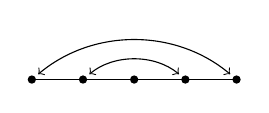
\begin{tikzpicture}[x=0.65cm,y=0.65cm,baseline=-2pt]
\draw (0,0)--(4,0);
\foreach \x in {0,1,2,3,4}{\fill (\x,0) circle (1.5pt);}
\draw[<->,shorten <=3pt,shorten >=3pt] (0,0) to[bend left=40] (4,0);
\draw[<->,shorten <=3pt,shorten >=3pt] (1,0) to[bend left=40] (3,0);
\end{tikzpicture}\\[12pt]
$D_4$ &
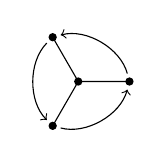
\begin{tikzpicture}[x=0.65cm,y=0.65cm,baseline=-2pt]
\draw (2,0)--(1.5,0.866) (2,0)--(1.5,-0.866) (2,0)--(3,0);
\foreach \p in {(2,0),(1.5,0.866),(1.5,-0.866),(3,0)}{\fill \p circle (1.5pt);}
\draw[->,shorten <=3pt,shorten >=3pt] (1.5,0.866) to[bend right=45] (1.5,-0.866);
\draw[->,shorten <=3pt,shorten >=3pt] (1.5,-0.866) to[bend right=45] (3,0);
\draw[->,shorten <=3pt,shorten >=3pt] (3,0) to[bend right=45] (1.5,0.866);
\end{tikzpicture}\\[12pt]
$D_n,\ n\geq5$ &
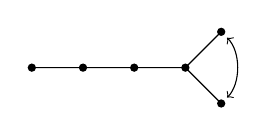
\begin{tikzpicture}[x=0.65cm,y=0.65cm,baseline=-2pt]
\draw (0,0)--(3,0)--(3.7,0.7) (3,0)--(3.7,-0.7);
\foreach \p in {(0,0),(1,0),(2,0),(3,0),(3.7,0.7),(3.7,-0.7)}{\fill \p circle (1.5pt);}
\draw[<->,shorten <=3pt,shorten >=3pt] (3.7,0.7) to[bend left=45] (3.7,-0.7);
\end{tikzpicture}\\[12pt]
$E_6$ &
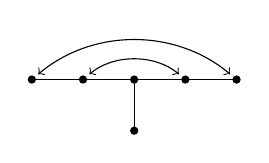
\begin{tikzpicture}[x=0.65cm,y=0.65cm,baseline=-2pt]
\draw (0,0)--(4,0) (2,0)--(2,-1);
\foreach \p in {(0,0),(1,0),(2,0),(3,0),(4,0),(2,-1)}{\fill \p circle (1.5pt);}
\draw[<->,shorten <=3pt,shorten >=3pt] (0,0) to[bend left=40] (4,0);
\draw[<->,shorten <=3pt,shorten >=3pt] (1,0) to[bend left=40] (3,0);
\end{tikzpicture}
\end{tabular}
\end{center}
（查看分类可知，连同 $n$ 为偶数时的 $A_n$，这些确实就是所有 $E/W$ 非平凡的情形。）

设 $S$ 是一个\Term{simple-root-system}{单根系}，暂不对其编号。已知 $E$ 是 $W$ 与保持 \Term{cartan-matrix}{Cartan 矩阵}（或 Dynkin 图，二者\Term{equivalence}{等价}）的 $S$ 的置换所成的群 $\Psi$ 的\Term{semidirect-product}{半直积}。群 $E/W$ 因而与 $\Psi$ 认同，特别地，$\varphi$ 对应于某个元素 $\psi\in\Psi$。查看 Dynkin 图（见上图）可以发现，$\psi$ 在 $S$ 中的每条\Term{orbit}{轨道}都由两两\Term{orthogonality}{正交}的\Term{root}{根}构成（即在图中不相连）。［注意，当 $R$ 为 $A_n$ 型且 $n$ 为偶数时，这一点不成立，因此必须单独处理该情形。］若 $\sigma$ 是这样一条\Term{orbit}{轨道}，则各反射 $r_a$（$a\in\sigma$）两两可交换；将它们的乘积记为 $\rho_\sigma$。显然 $\rho_\sigma$ 与 $\psi$ 可交换。

现在在 $S$ 上选一个\Term{totally-ordered}{全序}，使每条\Term{orbit}{轨道}对这个\Term{order-relation}{序关系}都是一个区段；这\Term{equivalence}{等价}于对 $S$ 的元素编号：$S=\{a_1,\ldots,a_n\}$。令 $\theta_1,\ldots,\theta_n$ 为前面定义的\Term{root}{根}，$c=r_1\cdots r_n$ 为相应的\Term{coxeter-element}{Coxeter 元素}。元素 $c$ 是各 $\rho_\sigma$ 按某个次序排列后的乘积，故它与 $\psi$ 可交换。置 $f=c\psi$。还可注意到 $\psi$ 将各 $\theta_i$ 互相置换。事实上，$\theta_i>0$，故 $\psi(\theta_i)>0$，且
\[c\bigl(\psi(\theta_i)\bigr)=\psi\bigl(c(\theta'_i)\bigr)<0,\]
所以由\Term{lemma}{引理} 5 (c)，$\psi(\theta_i)$ 等于某个 $\theta_j$。现在立即可见，
\SourcePage{253}
$f=c\psi$ 满足要求。事实上，若 $a\in R$，则有某对 $(m,i)$ 使 $a=c^m\theta_i$，从而对某个 $j$ 有 $a=f^m(\psi^{-m}\theta_i)=f^m\theta_j$。证毕。

\textbf{注记。} 可以证明，除情形 (2) 外，$f$ 的每条\Term{orbit}{轨道}都恰有 $h=\operatorname{Card}(R)/n$ 个元素，且包含唯一一个 $\theta_i$。在情形 (2) 中，有些 $\theta_i$ 是多余的。
\SourcePage{254}
% 原 PDF 第 254 页为空白页。
